\documentclass[conference]{IEEEtran}
\IEEEoverridecommandlockouts
\usepackage{cite}
\usepackage{amsmath,amssymb,amsfonts}
\usepackage{algorithmic}
\usepackage{graphicx}
\usepackage{textcomp}
\usepackage{xcolor}
\usepackage{booktabs}
\usepackage{multirow}
\usepackage{array}
\usepackage{tikz}
\usetikzlibrary{shapes.geometric, arrows.meta, positioning, fit,
                backgrounds, calc, decorations.pathreplacing}

\tikzset{
  proc/.style={rectangle, rounded corners=2pt, draw=black, thick,
               fill=blue!10, text width=3.0cm, align=center,
               minimum height=0.55cm, font=\scriptsize},
  sproc/.style={rectangle, rounded corners=2pt, draw=black, thick,
                fill=blue!10, text width=2.2cm, align=center,
                minimum height=0.52cm, font=\scriptsize},
  dec/.style={diamond, aspect=2.2, draw=black, thick, fill=yellow!20,
              text width=2.0cm, align=center, font=\scriptsize},
  db/.style={cylinder, shape border rotate=90, draw=black, thick,
             fill=green!15, minimum height=0.55cm, minimum width=1.8cm,
             align=center, font=\scriptsize},
  oval/.style={ellipse, draw=black, thick, fill=gray!20,
               minimum height=0.52cm, minimum width=1.6cm,
               align=center, font=\scriptsize},
  arr/.style={-{Stealth[length=4pt]}, thick},
  darr/.style={-{Stealth[length=4pt]}, thick, dashed},
  src/.style={rectangle, rounded corners=2pt, draw=black,
              fill=orange!15, text width=1.9cm, align=center,
              minimum height=0.50cm, font=\scriptsize},
  out/.style={rectangle, rounded corners=2pt, draw=black, thick,
              fill=green!15, text width=3.0cm, align=center,
              minimum height=0.52cm, font=\scriptsize},
  feat/.style={rectangle, draw=black, fill=purple!10,
               text width=2.0cm, align=center,
               minimum height=0.50cm, font=\scriptsize},
}

\def\BibTeX{{\rm B\kern-.05em{\sc i\kern-.025em b}\kern-.08em
    T\kern-.1667em\lower.7ex\hbox{E}\kern-.125emX}}

\begin{document}

\title{AI-Driven Epilepsy Genetic Variant Classification With ACMG
       Criteria and Retrieval-Augmented Generation}

\author{
\IEEEauthorblockN{Dr. M P Pushpalatha}
\IEEEauthorblockA{\textit{Dept. of Computer Science \& Eng.} \\
\textit{JSS Science and Technology University}\\
Mysuru, India \\
mppvin@jssstuniv.in}
\and
\IEEEauthorblockN{Srinidhi S G}
\IEEEauthorblockA{\textit{Dept. of Computer Science \& Eng.} \\
\textit{JSS Science and Technology University}\\
Mysuru, India \\
srinidhisg1@gmail.com}
\and
\IEEEauthorblockN{Bharath H}
\IEEEauthorblockA{\textit{Dept. of Computer Science \& Eng.} \\
\textit{JSS Science and Technology University}\\
Mysuru, India \\
bharath62004@gmail.com}
\and
\IEEEauthorblockN{Sushant Kabbinada}
\IEEEauthorblockA{\textit{Dept. of Computer Science \& Eng.} \\
\textit{JSS Science and Technology University}\\
Mysuru, India \\
sushant.k2150@gmail.com}
\and
\IEEEauthorblockN{Aditya Patil}
\IEEEauthorblockA{\textit{Dept. of Computer Science \& Eng.} \\
\textit{JSS Science and Technology University}\\
Mysuru, India \\
adityapatil0275@gmail.com}
}

\maketitle

% ═══════════════════════════════════════════════════════════════════════════════
\begin{abstract}
Classifying epilepsy genetic variants at scale requires a system
that is simultaneously fast, evidence-grounded, and self-contained.
We present a ten-layer diagnostic pipeline that accepts seven
clinician-entered fields (gene, chromosome, alleles, consequence,
variant type, and review status), expands them into 93 engineered
features, and scores them with an isotonic-calibrated XGBoost
classifier. On 7,673 held-out ClinVar variants across 26 epilepsy
genes the classifier attains 89.89\% accuracy, AUC 0.9446, F1
0.8538, and Brier score 0.0761. A central design choice is the
recycling of the classifier's own TreeSHAP attributions to satisfy
the ACMG PP3/BP4 computational-evidence criterion, eliminating
dependence on SIFT or PolyPhen-2; the resulting 14-criterion ACMG
engine agrees with 200 expert-panel ClinVar labels at 98.5\%.
When a variant is flagged pathogenic or uncertain
($\hat{p} \in [0.3, 0.7]$), four evidence fetchers (ClinVar,
gnomAD, PubMed via FAISS, PharmGKB) execute in parallel; a
four-voter adjudicator resolves ambiguity, a contradiction detector
flags inter-source conflicts, and Qwen3-32B synthesises a
structured clinical narrative. Total wall-clock time stays within
ten seconds without requiring any phenotype input. The maximum
cross-fold metric gap is 0.007. This system is intended for
research use only and has not been prospectively validated.
\end{abstract}

\begin{IEEEkeywords}
epilepsy, variant pathogenicity, XGBoost, ACMG/AMP, SHAP,
retrieval-augmented generation, large language model, clinical genomics
\end{IEEEkeywords}

% ═══════════════════════════════════════════════════════════════════════════════
\section{Introduction}

Epilepsy affects an estimated fifty million individuals worldwide
\cite{scheffer2017}. Clinical genomics has responded with expanded
gene-panel sequencing and whole-exome testing, yet many of the
variants discovered within known epilepsy genes carry no
established pathogenicity label---a gap documented at scale by the
Epi25 consortium across 17,606 sequenced individuals
\cite{epi25_2019}.

The ACMG/AMP five-tier classification framework \cite{richards2015}
provides a structured basis for interpreting these variants, but
applying it manually is labour-intensive: each case demands
population-frequency look-ups, inspection of prior clinical
submissions, review of functional evidence, and reconciliation of
all findings under a layered rule system. Nolan et al.\
\cite{nolan2022} illustrate the scale of this challenge through
a large-cohort multigene panel study in which a substantial
fraction of identified variants carried uncertain or ambiguous
clinical significance, underscoring the need for systematic and
reproducible classification workflows.

Existing automation tools address only fragments of this problem.
InterVar \cite{intervar2017} translates the ACMG decision logic
into Boolean rules but depends on SIFT and PolyPhen-2 to satisfy
the computational-evidence criterion (PP3/BP4)---services that are
subject to rate-limits and occasional downtime. AutoPVS1
\cite{autopvs1_2020} is narrowly scoped to a single criterion, PVS1.
Genome-wide deleteriousness scorers such as CADD \cite{cadd2014}
and REVEL \cite{revel2016} were not designed with epilepsy-specific
variant biology in mind. Nicora et al.\ \cite{nicora2022} treated
ACMG evidence tallies as input features for a random forest,
producing a useful prediction but no clinical narrative and
requiring phenotype data the system cannot source on its own.

No existing tool jointly (1) derives its own computational-evidence
criterion from the model's explainability output, (2) queries live
genomic databases at inference time to enrich each prediction, and
(3) synthesises a human-readable clinical report via a language
model. Our pipeline does all three. Specifically, our
contributions are:

\begin{itemize}
  \item An isotonic-calibrated XGBoost classifier that accepts
        seven clinical input fields and outputs a calibrated
        pathogenicity probability, trained on 52,323 ClinVar
        germline variants from 26 epilepsy genes.
  \item A 14-criterion ACMG engine where TreeSHAP values from
        our own classifier fill the PP3 and BP4 evidence slots.
        This removes the need for SIFT/PolyPhen-2 calls. A
        26-gene dictionary separates loss-of-function genes
        (22 genes, including SCN1A and CDKL5) from
        gain-of-function genes (SCN2A, SCN3A, SCN8A, SCN9A) to gate
        PVS1 correctly. The engine matches expert-panel labels
        on 197 out of 200 test variants.
  \item A retrieval-augmented generation layer that only fires
        when the variant is flagged pathogenic or uncertain
        ($\hat{p}\!\in\![0.3,0.7]$). Four fetchers (ClinVar
        REST, gnomAD GraphQL, PubMed via FAISS, PharmGKB) run
        through \texttt{asyncio.gather()}, a confidence resolver
        handles ambiguity, a contradiction detector catches
        disagreements, and Qwen3-32B via Groq produces a
        structured report. No phenotype input is needed.
\end{itemize}

% ═══════════════════════════════════════════════════════════════════════════════
\section{Related Work}

\subsection{Computational Pathogenicity Predictors}

SIFT and PolyPhen-2 gauge the functional impact of amino-acid
substitutions through evolutionary conservation; both remain
widely cited despite their restricted scope. CADD \cite{cadd2014}
generalised this idea by aggregating heterogeneous genomic
annotations into a unified deleteriousness score that spans all
variant classes. REVEL \cite{revel2016} extended the ensemble
approach further still, blending the outputs of multiple component
predictors into a meta-score that outperforms individual tools
on held-out rare missense variants.

For the structured, tabular feature representation our pipeline
uses, gradient-boosted trees have repeatedly matched or surpassed
deep learning across genomics benchmarks \cite{parente2021}.
XGBoost \cite{chen2016xgboost} was therefore a natural fit---not
merely on performance grounds, but because it natively produces
TreeSHAP attributions that our ACMG feedback loop requires.

\subsection{ACMG/AMP Automation Tools}

InterVar \cite{intervar2017} formalised the ACMG decision process
as a deterministic set of 28 Boolean rules, making it reproducible
but inflexible when external dependencies (SIFT, PolyPhen-2) are
unavailable. AutoPVS1 \cite{autopvs1_2020} targeted the PVS1
criterion alone, using transcript-level annotations to judge
loss-of-function consequences. Nicora et al.\ \cite{nicora2022}
reframed the problem: rather than encoding ACMG rules explicitly,
they used ACMG evidence tallies as input features for a random
forest classifier.

Our approach differs structurally from all three. Instead of
consulting external pathogenicity scorers for PP3/BP4, we route
our own classifier's SHAP attributions back into those evidence
slots---creating a closed, self-contained feedback loop. We also
introduce a gene-mechanism dictionary that labels each of our 26
panel genes as LOF or GOF, gating PVS1 appropriately. This is
essential because the four sodium-channel genes that act through
GOF (SCN2A, SCN3A, SCN8A, SCN9A) are not expected to cause disease
via protein truncation, and mistakenly awarding PVS1 there would
inflate the pathogenicity score without biological justification.

\subsection{Model Interpretability in Genomics}

The SHAP framework \cite{lundberg2017shap} decomposes each
prediction into signed per-feature contributions that sum exactly
to the model output, satisfying consistency and local-accuracy
axioms. This mathematical grounding makes attributions directly
comparable across variants. The TreeSHAP algorithm
\cite{lundberg2020trees} computes exact SHAP values for tree
ensembles in polynomial time, enabling attribution at every inference
call without a noticeable latency penalty. Watson \cite{watson2022}
documented the growing expectation in clinical genomics that
predictions be accompanied by feature-level explanations that
practitioners can interrogate.

\subsection{Retrieval-Augmented Generation}

Lewis et al.\ \cite{lewis2020rag} introduced retrieval-augmented
generation (RAG) as a method for grounding language model outputs
in documents fetched at query time, achieving markedly lower
hallucination rates than closed-book baselines on knowledge-intensive
tasks. In clinical NLP, BiomedRAG \cite{biomedrag2024} showed that
pairing a domain-specific retrieval index---built on PubMedBERT
\cite{pubmedbert2021} embeddings---with a biomedical corpus yields
substantially stronger performance on clinical question-answering
benchmarks than general-purpose retrieval pipelines.

% ═══════════════════════════════════════════════════════════════════════════════
\section{Dataset}

\subsection{Gene Panel and Data Collection}

Our gene panel comprises 26 loci retrieved from ClinVar
\cite{clinvar2018} on the basis of well-established causal links
to epilepsy. The selection spans the principal ion-channel
families: five voltage-gated sodium-channel genes (SCN1A, SCN2A,
SCN3A, SCN8A, SCN9A), two potassium-channel genes (KCNQ2, KCNQ3),
two GABA-receptor genes (GABRA1, GABRG2), four mTOR-pathway genes
(TSC1, TSC2, DEPDC5, NPRL3), and additional neurodevelopmental loci
(CDKL5, MECP2, STXBP1, PCDH19, FOXG1, SLC2A1, SLC6A1,
ARX, TBC1D24, PLCB1, CHD2, PRRT2, ALDH7A1).
Table~\ref{tab:genepanel} (Section~\ref{sec:acmg}) maps each gene
to its established clinical syndrome, seizure phenotype, typical
age of onset, molecular mechanism, and disease severity.

Only germline submissions with a definitive ClinVar label were
retained: Pathogenic and Likely Pathogenic were mapped to class 1;
Benign and Likely Benign to class 0. Variants of Uncertain
Significance were excluded entirely---their ambiguous clinical
status makes them unsuitable as training supervision.

\subsection{Preprocessing and Data Partitioning}

An inspection of the collected data revealed that 5$'$/3$'$ UTR
records exhibit a consequence distribution that diverges from
coding-region variants within the same gene, introducing
systematic label noise. We removed these 1,263 UTR entries,
leaving 52,323 analysable variants.

The cleaned dataset was partitioned using stratified sampling into
training (70\%, 35,718 variants), validation (15\%, 7,669), and
test (15\%, 7,673) folds. The raw pathogenic-to-benign ratio is
approximately 2:1. To address this imbalance we applied SMOTE
combined with Tomek link removal exclusively to the training fold,
expanding it to 44,644 samples. The validation and test folds
were left untouched throughout---a deliberate choice to ensure
that synthetic oversampling did not inflate held-out evaluation
scores. Fig.~\ref{fig:datapipeline} shows the full pipeline
with decision gates and record counts at each stage.
Fig.~\ref{fig:classsmote} shows the class-balance shift after
resampling and the per-gene variant distribution across all 26
genes.

\begin{figure}[!htb]
\centering
\resizebox{\columnwidth}{!}{%
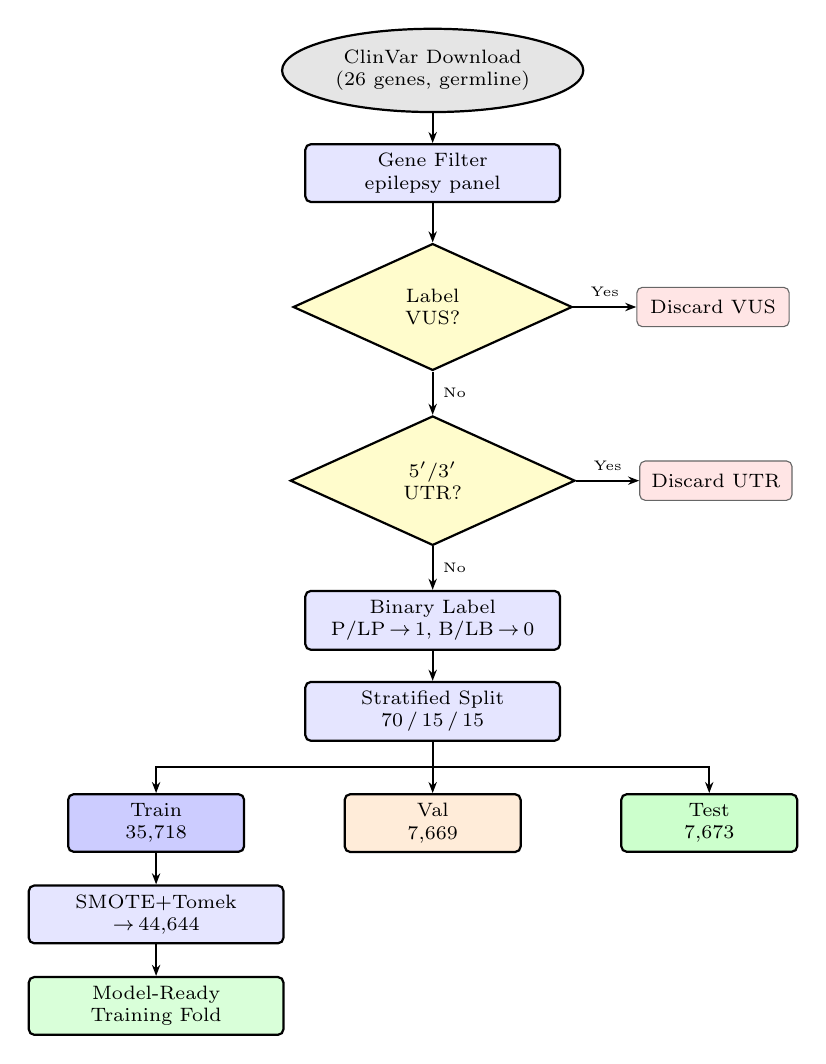
\begin{tikzpicture}[
    node distance=0.38cm and 0.30cm,
    st/.style  ={rectangle, rounded corners=2pt, draw=black, thick,
                 fill=blue!10, text width=3.0cm, align=center,
                 minimum height=0.55cm, font=\scriptsize},
    dec2/.style={diamond, aspect=2.2, draw=black, thick, fill=yellow!20,
                 text width=1.8cm, align=center, font=\scriptsize},
    dis/.style ={rectangle, rounded corners=2pt, draw=black!60,
                 fill=red!10, text width=1.7cm, align=center,
                 minimum height=0.50cm, font=\scriptsize},
    trn/.style ={rectangle, rounded corners=2pt, draw=black, thick,
                 fill=blue!20, text width=2.0cm, align=center,
                 minimum height=0.52cm, font=\scriptsize},
    val2/.style={rectangle, rounded corners=2pt, draw=black, thick,
                 fill=orange!15, text width=2.0cm, align=center,
                 minimum height=0.52cm, font=\scriptsize},
    tst/.style ={rectangle, rounded corners=2pt, draw=black, thick,
                 fill=green!20, text width=2.0cm, align=center,
                 minimum height=0.52cm, font=\scriptsize},
    out2/.style ={rectangle, rounded corners=2pt, draw=black, thick,
                 fill=green!15, text width=3.0cm, align=center,
                 minimum height=0.52cm, font=\scriptsize},
  ]
  \node[oval]   (start) {ClinVar Download\\(26 genes, germline)};
  \node[st,  below=of start]         (gf)     {Gene Filter\\epilepsy panel};
  \node[dec2,below=0.5cm of gf]      (vusdec) {Label\\VUS?};
  \node[dis, right=0.8cm of vusdec]  (vusdis) {Discard VUS};
  \node[dec2,below=0.55cm of vusdec] (utrdec) {5$'$/3$'$\\UTR?};
  \node[dis, right=0.8cm of utrdec]  (utrdis) {Discard UTR};
  \node[st,  below=0.55cm of utrdec] (label)  {Binary Label\\P/LP\,$\to$\,1,\;B/LB\,$\to$\,0};
  \node[st,  below=of label]         (split)  {Stratified Split\\70\,/\,15\,/\,15};
  \node[trn, below left=0.65cm and 0.75cm of split] (train){Train\\35,718};
  \node[val2,below=0.65cm of split]                 (val)  {Val\\7,669};
  \node[tst, below right=0.65cm and 0.75cm of split](test) {Test\\7,673};
  \node[st,  below=0.4cm of train]  (smote){SMOTE+Tomek\\$\to$\,44,644};
  \node[out2,below=0.4cm of smote]  (ready){Model-Ready\\Training Fold};
  \draw[arr](start)--(gf);
  \draw[arr](gf)--(vusdec);
  \draw[arr](vusdec.east)--node[above,font=\tiny]{Yes}(vusdis);
  \draw[arr](vusdec.south)--node[right,font=\tiny]{No}(utrdec);
  \draw[arr](utrdec.east)--node[above,font=\tiny]{Yes}(utrdis);
  \draw[arr](utrdec.south)--node[right,font=\tiny]{No}(label);
  \draw[arr](label)--(split);
  \draw[arr](split.south)--++(0,-0.32)-|(train.north);
  \draw[arr](split.south)--++(0,-0.32)--(val.north);
  \draw[arr](split.south)--++(0,-0.32)-|(test.north);
  \draw[arr](train)--(smote);
  \draw[arr](smote)--(ready);
\end{tikzpicture}%
}
\caption{Data pipeline. Decision diamonds remove VUS (no clean label)
         and UTR records (label noise), leaving 52,323 variants.
         A stratified 70/15/15 split is applied; SMOTE+Tomek
         resampling runs on the training fold only.}
\label{fig:datapipeline}
\end{figure}

\begin{figure}[!htb]
\centering
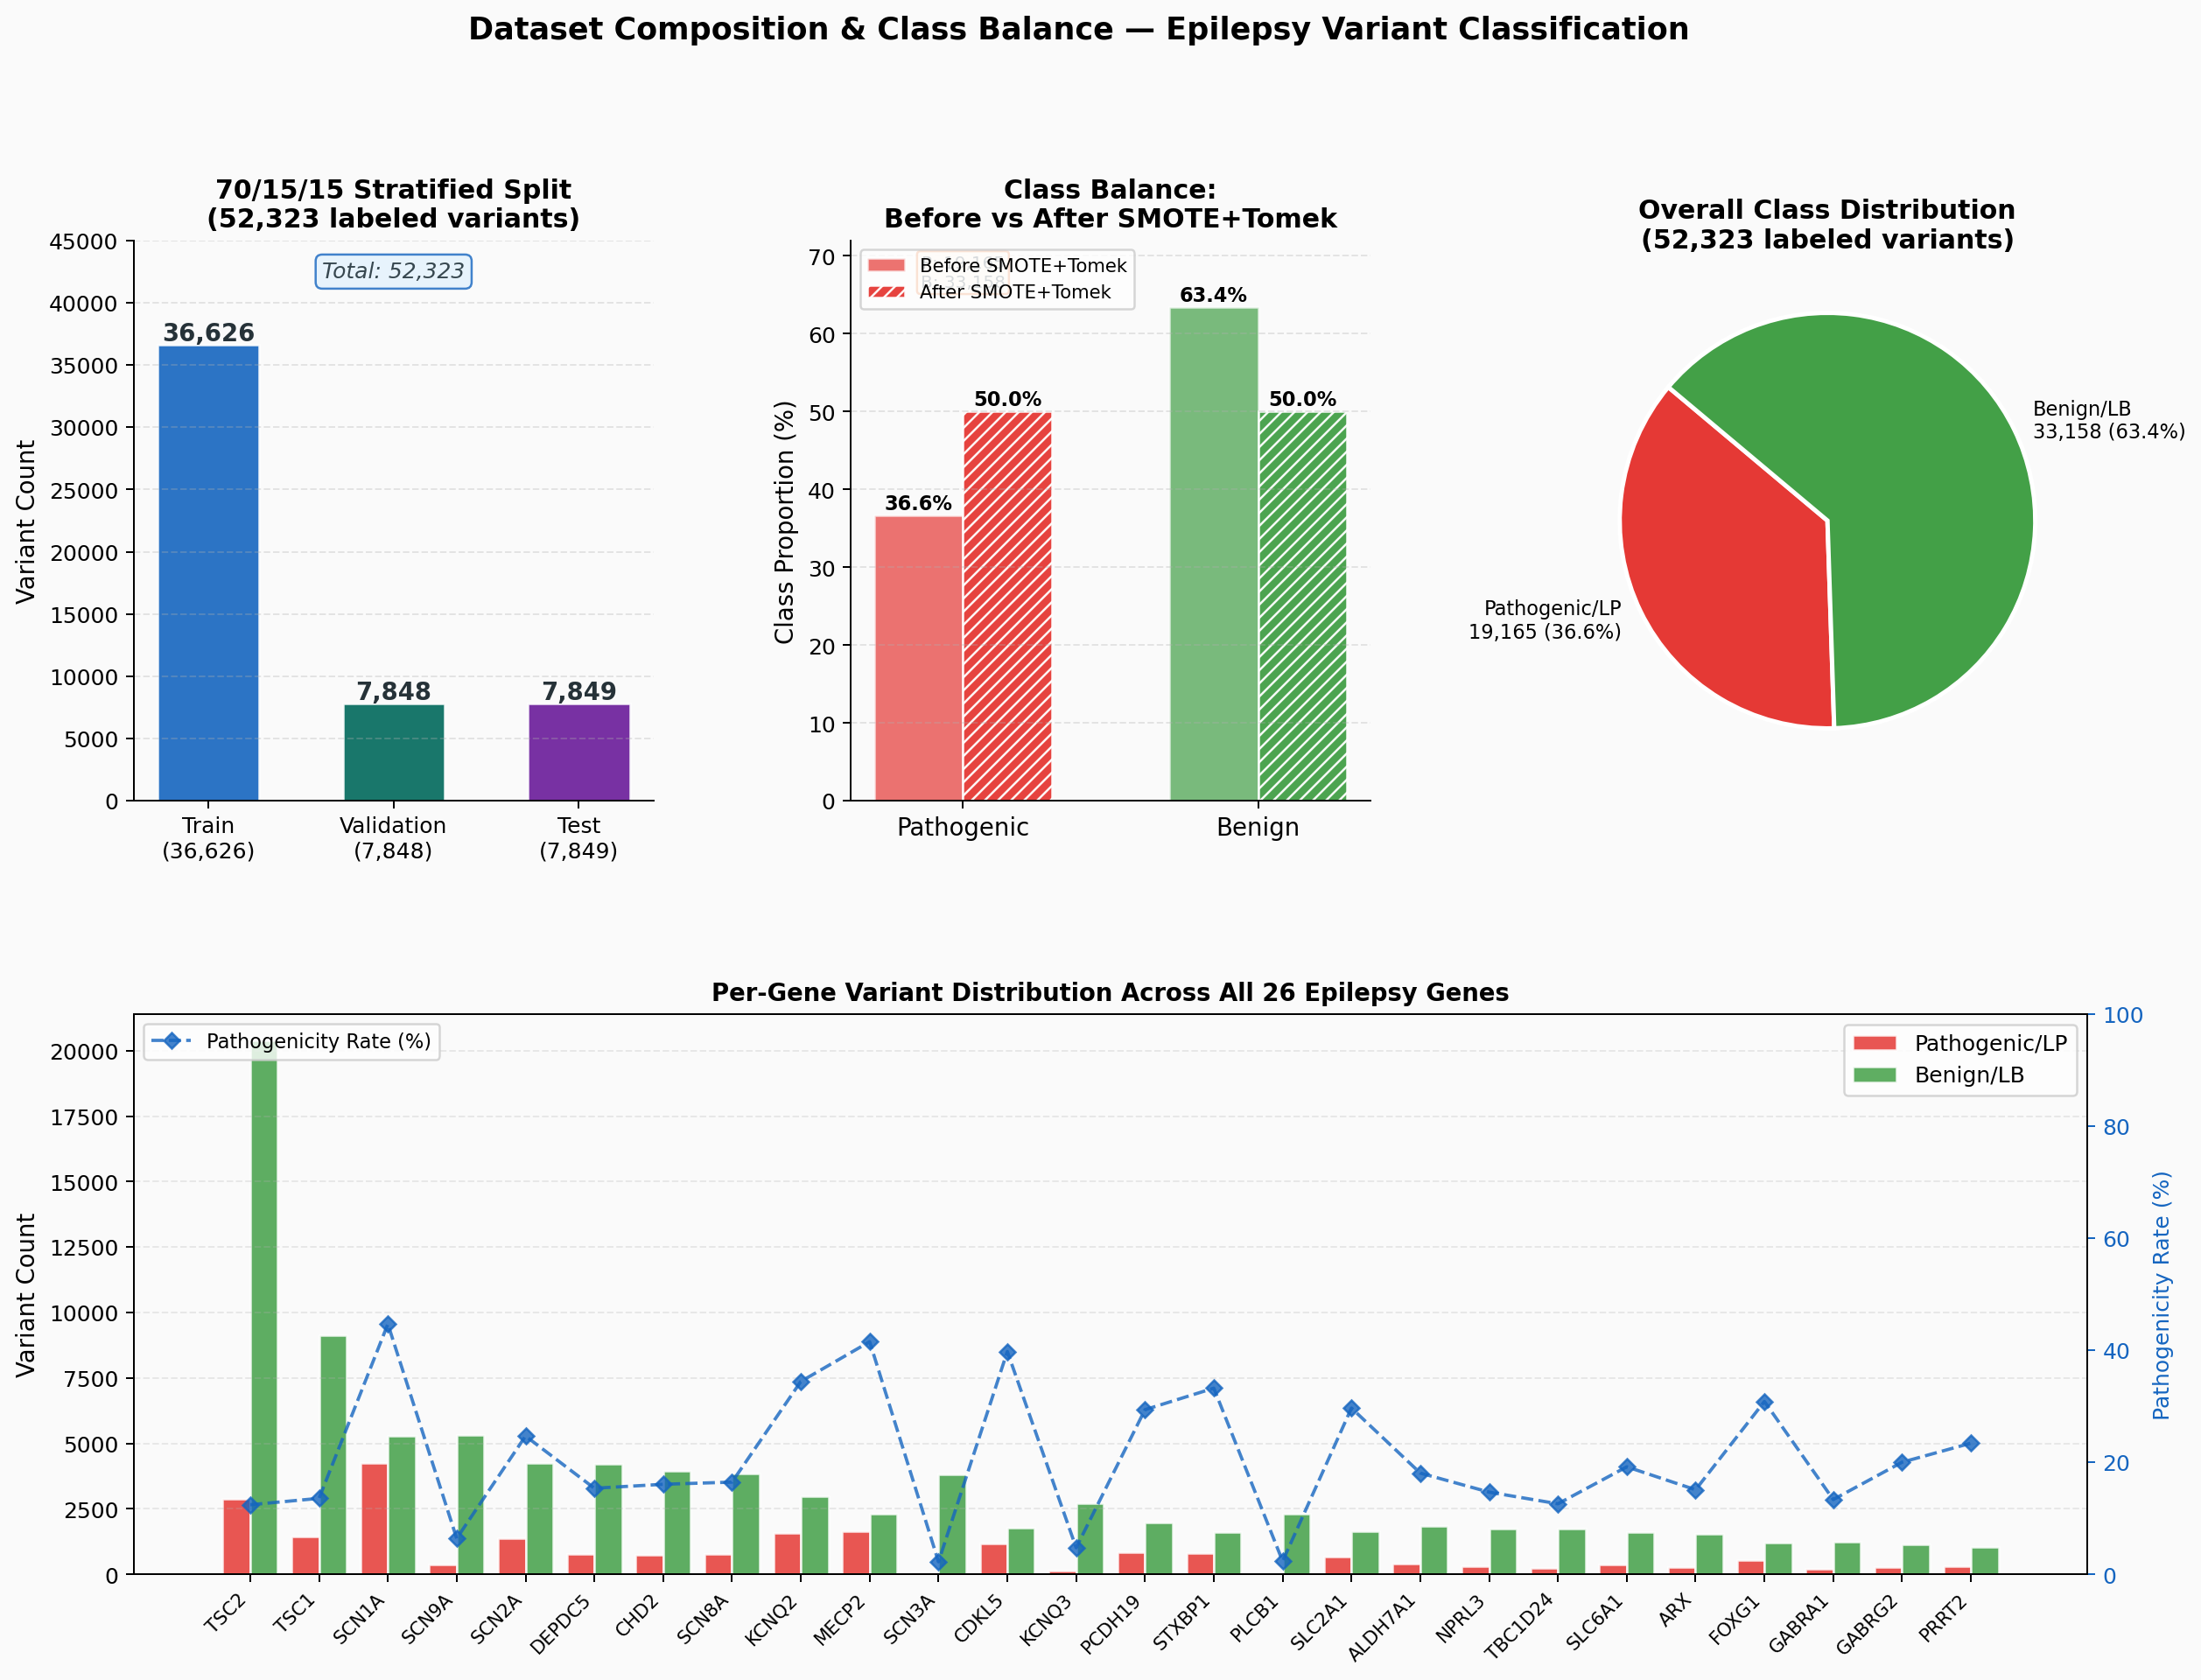
\includegraphics[width=\columnwidth]{fig7_class_distribution_smote_genes.png}
\caption{Left: class counts before and after SMOTE+Tomek resampling.
         The training fold expands from 35,718 to 44,644 samples.
         Validation and test folds are untouched. Right: per-gene
         variant counts across the 26-gene panel. SCN1A and MECP2
         have the most entries; PRRT2 and TBC1D24 the fewest.}
\label{fig:classsmote}
\end{figure}

% ═══════════════════════════════════════════════════════════════════════════════
\section{Proposed Methodology}

\subsection{Feature Engineering Pipeline}

The pipeline transforms each variant through three data shapes.

\textbf{Shape~1 --- Validated input.}
Every request enters through a Pydantic schema called
\texttt{VariantInput} that requires seven fields: \texttt{gene},
\texttt{chromosome}, \texttt{reference\_allele},
\texttt{alternate\_allele}, \texttt{consequence},
\texttt{variant\_type}, and \texttt{review\_status}. There is also
an optional \texttt{position} integer. If the input is malformed,
the API returns HTTP~422 immediately. We picked Pydantic over
hand-written checks because it gives us automatic type coercion
and clear error messages at the API boundary, which helps prevent
bad allele strings from silently propagating downstream.

\textbf{Shape~2 --- 93-dimensional feature vector.}
A stateless function called \texttt{engineer\_features()} takes
the seven fields and produces a 93-column numeric vector. We
deliberately chose deterministic offline features instead of
learned embeddings for two practical reasons. First, the same
input always gives the same vector, regardless of whether external
APIs are up or down. Second, every single column is directly
interpretable through SHAP---this would not be possible with
opaque embedding dimensions, and we need meaningful SHAP values
for the PP3/BP4 feedback loop.

The 93 columns break down into nine groups
(Table~\ref{tab:featuregroups}):

\begin{itemize}
  \item \textbf{Gene identity} (26 one-hot columns, one per gene).
  \item \textbf{Gene family flags} (4 binary:
        \texttt{is\_sodium\_channel}, \texttt{is\_ion\_channel},
        \texttt{is\_gaba\_receptor}, \texttt{is\_tsc\_complex}).
        These capture channel-class membership so that the model
        can learn shared patterns across, e.g., all sodium-channel
        genes.
  \item \textbf{Gene-level statistics} (2 real-valued:
        \texttt{gene\_pathogenicity\_rate} and
        \texttt{gene\_sample\_count}). These are pre-computed from
        the training fold and stored in a JSON file loaded at
        server startup---so there is no label leakage at inference
        time. If a gene was not seen in training, both default
        to 0.5.
  \item \textbf{Molecular consequence flags} (9 binary: including
        \texttt{is\_frameshift}, \texttt{is\_nonsense},
        \texttt{is\_splice}, \texttt{is\_missense},
        \texttt{is\_synonymous}, and a composite
        \texttt{severe\_consequence\_count} that tallies how many
        of the severe flags are active simultaneously).
  \item \textbf{Variant-type indicators} (17: one-hot encoding of
        12 variant types plus 5 binary flags like \texttt{is\_snp},
        \texttt{is\_deletion}).
  \item \textbf{Allele/position features} (8: derived from
        string-length arithmetic on the reference and alternate
        allele fields---\texttt{ref\_length}, \texttt{alt\_length},
        \texttt{allele\_length\_diff}, etc.).
  \item \textbf{Chromosome one-hots} (15 columns).
  \item \textbf{Review-status ordinals} (6: including
        \texttt{review\_score} mapped to 0--4,
        \texttt{has\_expert\_review}, and
        \texttt{has\_multiple\_submitters}).
  \item \textbf{Nucleotide-context flags} (6:
        \texttt{is\_transition}, \texttt{is\_transversion},
        \texttt{is\_grch38}, \texttt{is\_grch37}, etc.).
\end{itemize}

One implementation detail worth noting: at inference time, if the
trained model expects a column that is missing from the generated
vector (e.g., a chromosome value not seen during training produces
no one-hot match), the pipeline fills it with zero and reorders all
columns to match the training-time sequence. This prevents crashes
on unexpected inputs. Fig.~\ref{fig:featpipeline} illustrates the
mapping.

\begin{figure}[!htb]
\centering
\begin{tikzpicture}[node distance=0.30cm and 0.22cm]
  \node[sproc, fill=gray!15]  (inp) {7-Field VariantInput};
  \node[feat, below left=0.55cm and -0.3cm of inp]  (g1) {Gene one-hot\\(26)};
  \node[feat, right=0.18cm of g1]                   (g2) {Gene family\\flags (4)};
  \node[feat, below=0.22cm of g1]                   (g3) {Gene stats\\(2)};
  \node[feat, right=0.18cm of g3]                   (g4) {Consequence\\flags (9)};
  \node[feat, below=0.22cm of g3]                   (g5) {Type flags\\+ one-hot (17)};
  \node[feat, right=0.18cm of g5]                   (g6) {Allele /\\position (8)};
  \node[feat, below=0.22cm of g5]                   (g7) {Chromosome\\one-hot (15)};
  \node[feat, right=0.18cm of g7]                   (g8) {Review\\status (6)};
  \node[feat, below=0.22cm of g7, xshift=1.15cm]    (g9) {Ti/Tv /\\assembly (6)};
  \node[out, below=0.55cm of g9, xshift=-1.15cm]   (vec) {93-dim vector\\(\texttt{pd.DataFrame})};
  \foreach \g in {g1,g2,g3,g4,g5,g6,g7,g8,g9} \draw[arr](inp)--(\g);
  \foreach \g in {g1,g2,g3,g4,g5,g6,g7,g8,g9} \draw[arr](\g)--(vec);
\end{tikzpicture}
\caption{Feature expansion. Seven clinical inputs become 93 numeric
         columns via nine semantic groups. No network call is needed.}
\label{fig:featpipeline}
\end{figure}

\begin{table}[!htb]
\caption{Breakdown of the 93 Engineered Features}
\label{tab:featuregroups}
\begin{center}
\begin{tabular}{lcc}
\toprule
\textbf{Group} & \textbf{Dims} & \textbf{Encoding} \\
\midrule
Gene identity (one-hot, 26 genes)             & 26 & Binary \\
Gene family (Na$^+$, K$^+$, GABA, TSC)       &  4 & Binary \\
Gene-level statistics                         &  2 & Real \\
Molecular consequence flags                   &  9 & Binary \\
Variant-type flags + one-hot                  & 17 & Binary \\
Allele / genomic-position                     &  8 & Integer \\
Chromosome (one-hot, 15 values)               & 15 & Binary \\
Review-status indicators                      &  6 & Ordinal/Real \\
Nucleotide context (Ti/Tv, assembly)          &  6 & Binary \\
\midrule
\textbf{Total}                                & \textbf{93} & \\
\bottomrule
\end{tabular}
\end{center}
\end{table}

\textbf{Shape~3 --- Composite prediction.}
The output is a JSON object called \texttt{PredictionResult}. It
contains: the binary label, the calibrated probability $\hat{p}$,
a six-level confidence tier, the ACMG classification with its
Tavtigian point total and triggered criteria list, per-feature SHAP
values, and (when the conditional path fires) the LLM-generated
clinical narrative. External evidence from ClinVar, gnomAD, and
PharmGKB is cached in per-source SQLite databases---30 days for
ClinVar and gnomAD, 24 hours for PubMed literature---to balance
freshness against API rate limits.

\subsection{System Design and Module Architecture}

We designed each pipeline stage as a single class with one public
method. This way, any stage can be tested in isolation, swapped out
for a different implementation, or skipped entirely.
Fig.~\ref{fig:ooflow} traces the full ten-class chain.

\begin{figure}[!htb]
\centering
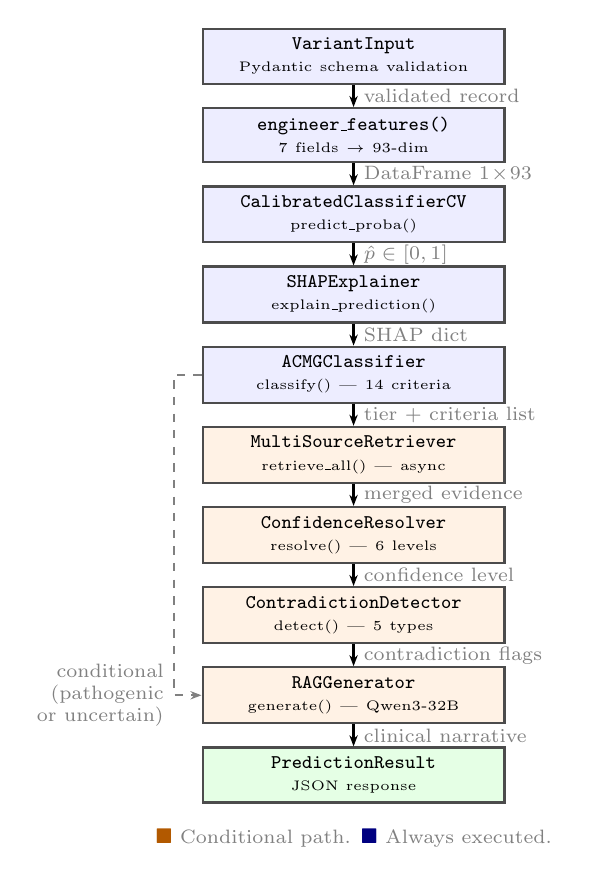
\begin{tikzpicture}[
    node distance=0.28cm and 0.20cm,
    cls/.style={rectangle, draw=black!70, thick, fill=blue!7,
                text width=3.6cm, align=center,
                minimum height=0.58cm, font=\scriptsize},
    cnd/.style={rectangle, draw=black!70, thick, fill=orange!10,
                text width=3.6cm, align=center,
                minimum height=0.58cm, font=\scriptsize},
    res/.style={rectangle, draw=black!70, thick, fill=green!10,
                text width=3.6cm, align=center,
                minimum height=0.58cm, font=\scriptsize},
    lbl/.style={font=\scriptsize, text=gray, align=center},
  ]
  \node[cls] (vi)  {\texttt{VariantInput}\\{\tiny Pydantic schema validation}};
  \node[cls, below=of vi]  (ef)  {\texttt{engineer\_features()}\\{\tiny 7 fields $\to$ 93-dim}};
  \node[cls, below=of ef]  (xgb) {\texttt{CalibratedClassifierCV}\\{\tiny predict\_proba()}};
  \node[cls, below=of xgb] (shp) {\texttt{SHAPExplainer}\\{\tiny explain\_prediction()}};
  \node[cls, below=of shp] (acm) {\texttt{ACMGClassifier}\\{\tiny classify() --- 14 criteria}};
  \node[cnd, below=of acm] (ret) {\texttt{MultiSourceRetriever}\\{\tiny retrieve\_all() --- async}};
  \node[cnd, below=of ret] (cr)  {\texttt{ConfidenceResolver}\\{\tiny resolve() --- 6 levels}};
  \node[cnd, below=of cr]  (cd)  {\texttt{ContradictionDetector}\\{\tiny detect() --- 5 types}};
  \node[cnd, below=of cd]  (rag) {\texttt{RAGGenerator}\\{\tiny generate() --- Qwen3-32B}};
  \node[res, below=of rag] (pr)  {\texttt{PredictionResult}\\{\tiny JSON response}};

  \draw[arr](vi) --node[right,lbl]{validated record}(ef);
  \draw[arr](ef) --node[right,lbl]{DataFrame $1\!\times\!93$}(xgb);
  \draw[arr](xgb)--node[right,lbl]{$\hat{p}\in[0,1]$}(shp);
  \draw[arr](shp)--node[right,lbl]{SHAP dict}(acm);
  \draw[arr](acm)--node[right,lbl]{tier + criteria list}(ret);
  \draw[arr](ret)--node[right,lbl]{merged evidence}(cr);
  \draw[arr](cr) --node[right,lbl]{confidence level}(cd);
  \draw[arr](cd) --node[right,lbl]{contradiction flags}(rag);
  \draw[arr](rag)--node[right,lbl]{clinical narrative}(pr);

  \draw[darr,color=gray](acm.west)--++(-0.35,0)
        |-node[left,font=\scriptsize,text=gray,align=right]
          {conditional\\(pathogenic\\or uncertain)}(rag.west);

  \node[below=0.20cm of pr, font=\scriptsize, text=gray, align=left]
    {\textcolor{orange!70!black}{$\blacksquare$}~Conditional path.
     \textcolor{blue!50!black}{$\blacksquare$}~Always executed.};
\end{tikzpicture}
\caption{Module chain. Blue boxes run on every request; orange
         boxes only activate for pathogenic or uncertain
         predictions ($\hat{p}\!\in\![0.3,0.7]$).}
\label{fig:ooflow}
\end{figure}

A key architectural decision was splitting the pipeline into an
unconditional path (Layers~1--5) and a conditional path
(Layers~6--9). During early prototyping we found that calling
ClinVar and gnomAD for every single variant---including obviously
benign synonymous changes---added 3--8 seconds of latency per
request and burned through the NCBI E-utilities rate limit (10
requests/second with an API key, 3/second without), all without
changing the classification outcome. So we gate the retrieval on
the classifier's confidence: only pathogenic or uncertain
predictions trigger the four parallel fetchers, the contradiction
detector, and the LLM report. Benign-confident variants exit after
ACMG scoring in under one second.

Fig.~\ref{fig:arch} shows the ten-layer stack, and
Fig.~\ref{fig:inferencepipeline} shows the branching inference path
with the four-way parallel fan-out.

\begin{figure}[!htb]
\centering
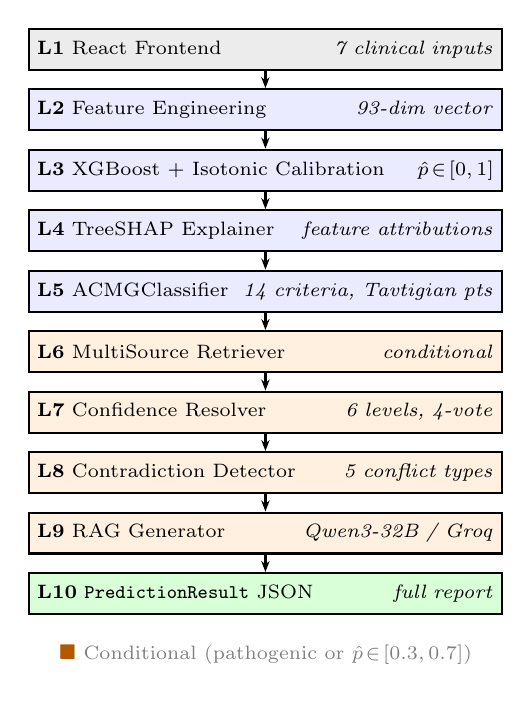
\begin{tikzpicture}[
    node distance=0.22cm,
    blk/.style={rectangle, draw=black, thick, fill=blue!8,
                text width=5.8cm, align=left, minimum height=0.52cm,
                font=\scriptsize, inner sep=3pt},
    out2/.style={rectangle, draw=black, thick, fill=green!15,
                 text width=5.8cm, align=left, minimum height=0.52cm,
                 font=\scriptsize, inner sep=3pt},
    inp/.style={rectangle, draw=black, thick, fill=gray!15,
                text width=5.8cm, align=left, minimum height=0.52cm,
                font=\scriptsize, inner sep=3pt},
    cnd/.style={rectangle, draw=black, thick, fill=orange!12,
                text width=5.8cm, align=left, minimum height=0.52cm,
                font=\scriptsize, inner sep=3pt},
  ]
  \node[inp]  (L1) {\textbf{L1}\ React Frontend \hfill \textit{7 clinical inputs}};
  \node[blk, below=of L1] (L2) {\textbf{L2}\ Feature Engineering \hfill \textit{93-dim vector}};
  \node[blk, below=of L2] (L3) {\textbf{L3}\ XGBoost + Isotonic Calibration \hfill $\hat{p}\!\in\![0,1]$};
  \node[blk, below=of L3] (L4) {\textbf{L4}\ TreeSHAP Explainer \hfill \textit{feature attributions}};
  \node[blk, below=of L4] (L5) {\textbf{L5}\ ACMGClassifier \hfill \textit{14 criteria, Tavtigian pts}};
  \node[cnd, below=of L5] (L6) {\textbf{L6}\ MultiSource Retriever \hfill \textit{conditional}};
  \node[cnd, below=of L6] (L7) {\textbf{L7}\ Confidence Resolver \hfill \textit{6 levels, 4-vote}};
  \node[cnd, below=of L7] (L8) {\textbf{L8}\ Contradiction Detector \hfill \textit{5 conflict types}};
  \node[cnd, below=of L8] (L9) {\textbf{L9}\ RAG Generator \hfill \textit{Qwen3-32B / Groq}};
  \node[out2,below=of L9] (L10){\textbf{L10}\ \texttt{PredictionResult} JSON \hfill \textit{full report}};
  \foreach \a/\b in {L1/L2,L2/L3,L3/L4,L4/L5,L5/L6,L6/L7,L7/L8,L8/L9,L9/L10}
    \draw[arr](\a)--(\b);
  \node[below=0.25cm of L10,font=\scriptsize,text=gray,align=left]
    {\textcolor{orange!70!black}{$\blacksquare$}~Conditional
     (pathogenic or $\hat{p}\!\in\![0.3,0.7]$)};
\end{tikzpicture}
\caption{Ten-layer stack. Layers~1--5 run always; Layers~6--9
         (orange) only fire for pathogenic or uncertain predictions.}
\label{fig:arch}
\end{figure}

\begin{figure}[!htb]
\centering
\begin{tikzpicture}[node distance=0.32cm and 0.20cm]
  \node[oval]  (req)  {HTTP POST \texttt{/predict}};
  \node[proc, below=of req] (val) {Pydantic Validation};
  \node[proc, below=of val] (feat){Feature Engineering (93-dim)};
  \node[proc, below=of feat](ml)  {XGBoost \texttt{predict\_proba()}};
  \node[proc, below=of ml]  (shap){TreeSHAP Attribution};
  \node[proc, below=of shap](acmg){ACMGClassifier \texttt{.classify()}};
  \node[dec,  below=of acmg](gate){Pathogenic\\or uncertain?};
  \node[out,  right=1.8cm of gate](resp){\texttt{PredictionResult}\\(fast path)};
  \node[src,  below left=0.7cm and 1.0cm of gate] (cv){ClinVar\\REST};
  \node[src,  below left=0.7cm and -0.2cm of gate](gn){gnomAD\\GraphQL};
  \node[src,  below right=0.7cm and -0.2cm of gate](pm){PubMed\\FAISS};
  \node[src,  below right=0.7cm and 1.0cm of gate](pk){PharmGKB\\REST};
  \node[proc, below=1.55cm of gate](merge){Merge Evidence};
  \node[proc, below=of merge]      (cr)  {Confidence Resolver};
  \node[proc, below=of cr]         (cd)  {Contradiction Detector};
  \node[proc, below=of cd]         (llm) {RAGGenerator (Qwen3-32B)};
  \node[out,  below=of llm]        (full){\texttt{PredictionResult}\\(full report)};
  \draw[arr](req)--(val); \draw[arr](val)--(feat); \draw[arr](feat)--(ml);
  \draw[arr](ml)--(shap); \draw[arr](shap)--(acmg); \draw[arr](acmg)--(gate);
  \draw[arr](gate.east)--node[above,font=\scriptsize]{No}(resp);
  \coordinate (fanout) at ($(gate.south)+(0,-0.35)$);
  \draw[arr](gate.south)--node[left,font=\scriptsize]{Yes}(fanout);
  \draw[arr](fanout)-|(cv.north);
  \draw[arr](fanout)-|(gn.north);
  \draw[arr](fanout)-|(pm.north);
  \draw[arr](fanout)-|(pk.north);
  \draw[arr](cv.south)|-(merge.west); \draw[arr](gn.south)|-(merge.west);
  \draw[arr](pm.south)|-(merge.east); \draw[arr](pk.south)|-(merge.east);
  \draw[arr](merge)--(cr); \draw[arr](cr)--(cd);
  \draw[arr](cd)--(llm); \draw[arr](llm)--(full);
  \node[db, right=0.5cm of cv, yshift=-0.5cm](cache){SQLite\\Cache};
  \draw[darr](cv.east)-|(cache.north);
  \draw[darr](gn.east)-|(cache.north);
\end{tikzpicture}
\caption{Branching inference flow. Benign-confident variants exit
         via the fast path. Pathogenic or uncertain ones fan out to
         four parallel fetchers, then go through confidence
         resolution, contradiction detection, and LLM synthesis.}
\label{fig:inferencepipeline}
\end{figure}

\textbf{How the retriever allocates context space.}
The \texttt{MultiSourceRetriever} divides its context budget across
sources: 40\% to ClinVar (variant-specific clinical evidence),
30\% to PharmGKB (drug--gene interactions for epilepsy medications),
10\% to gnomAD (population allele frequency), and 20\% to PubMed
(literature via FAISS nearest-neighbour search over PubMedBERT
\cite{pubmedbert2021} embeddings of epilepsy abstracts). ClinVar
gets the largest share because variant-specific clinical evidence
is the most directly actionable for ACMG classification.

\textbf{Confidence resolver.}
The \texttt{ConfidenceResolver} partitions the $\hat{p}$ axis into
six zones: very\_high ($\geq$\,0.9), high ($\geq$\,0.7),
moderate\_pathogenic ($\geq$\,0.5), moderate\_benign ($\geq$\,0.3),
high\_benign ($\geq$\,0.1), and very\_high\_benign ($<$\,0.1).
Variants in the uncertain band ($0.3 \leq \hat{p} \leq 0.7$) go
through a four-voter adjudication. Each voter contributes weighted
evidence: ClinVar entries with $\geq$\,2 review stars contribute up
to 2.5 pathogenic points; gnomAD frequency above 1\% contributes
1 benign point; severe consequences contribute 1.5 pathogenic
points; SHAP polarity is noted but not numerically scored. If
pathogenic evidence exceeds benign by more than 1, the resolver
suggests Likely Pathogenic; benign exceeds pathogenic by more
than 1, Likely Benign; otherwise VUS. Fig.~\ref{fig:confzones}
shows the zone layout.

\textbf{Contradiction detector.}
\texttt{ContradictionDetector} checks five conflict types:
(1)~ML-vs-ClinVar---high severity if ClinVar has $\geq$\,2 stars;
(2)~ML-vs-gnomAD---high severity if the variant is common
($\text{AF} > 0.01$);
(3)~ML-vs-consequence---medium severity when a benign prediction
coincides with a severe consequence like frameshift or stop-gained;
(4)~ClinVar internal conflict---when ClinVar itself has conflicting
interpretations from different submitters;
(5)~uncertainty analysis---a free-text summary of all evidence
injected into the LLM prompt.

\begin{figure}[!htb]
\centering
\resizebox{\columnwidth}{!}{%
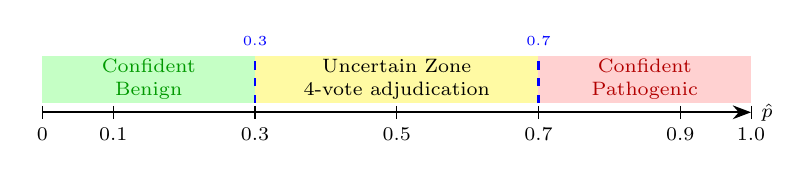
\begin{tikzpicture}
  % axis
  \draw[thick,{-Stealth}](0,0)--(9.0,0)
        node[right,font=\scriptsize]{$\hat{p}$};
  % tick marks
  \foreach \x/\lbl in {0/0, 0.9/0.1, 2.7/0.3, 4.5/0.5, 6.3/0.7, 8.1/0.9, 9.0/1.0}
    \draw(\x,0.08)--(\x,-0.08) node[below,font=\scriptsize]{\lbl};
  % coloured zones
  \fill[green!25,opacity=0.9](0,0.12)  rectangle(2.7,0.72);
  \fill[yellow!40,opacity=0.9](2.7,0.12) rectangle(6.3,0.72);
  \fill[red!20,opacity=0.9]  (6.3,0.12) rectangle(9.0,0.72);
  % zone labels
  \node[font=\scriptsize,text=green!60!black,align=center] at(1.35,0.42)
        {Confident\\Benign};
  \node[font=\scriptsize,align=center] at(4.50,0.42)
        {Uncertain Zone\\4-vote adjudication};
  \node[font=\scriptsize,text=red!70!black,align=center] at(7.65,0.42)
        {Confident\\Pathogenic};
  % threshold dashed lines (label inside bar to avoid vertical overlap)
  \draw[dashed,blue,thick](2.7,0.12)--(2.7,0.72);
  \draw[dashed,blue,thick](6.3,0.12)--(6.3,0.72);
  \node[font=\tiny,text=blue,above] at(2.7,0.72) {0.3};
  \node[font=\tiny,text=blue,above] at(6.3,0.72) {0.7};
\end{tikzpicture}%
}
\caption{Confidence zones along the pathogenic probability axis.
         Variants outside $[0.3,\,0.7]$ exit immediately; those
         inside trigger four-voter adjudication
         (gnomAD $\cdot$ ClinVar $\cdot$ SHAP $\cdot$ Consequence).}
\label{fig:confzones}
\end{figure}

% ═══════════════════════════════════════════════════════════════════════════════
\section{Classification Model}

\subsection{Model Selection and Training}

XGBoost \cite{chen2016xgboost} was chosen on two grounds. First,
prior genomics benchmarks show gradient-boosted trees match or
exceed deep networks on structured tabular data \cite{parente2021}.
Second, XGBoost natively supports TreeSHAP \cite{lundberg2020trees},
which runs in polynomial time per prediction and produces
feature-level attributions that are directly comparable across
variants. Deep-network attribution methods (e.g., Integrated
Gradients) carry no such consistency guarantee, making it
impossible to reliably threshold their outputs against fixed ACMG
criteria thresholds---a requirement our PP3/BP4 feedback loop
depends on.

Raw XGBoost probabilities were replaced with isotonic regression
estimates via \texttt{CalibratedClassifierCV} (five internal folds).
Sigmoid (Platt) scaling was also evaluated; it produced Brier 0.087
on the validation fold versus 0.076 for isotonic, so isotonic was
retained. High-confidence accuracy reached 96.4\% on the 65\% of
test samples whose $\hat{p}$ cleared the confidence boundary.

Hyperparameters fixed on the validation fold: max depth~8, learning
rate~0.05, 300 trees, subsample~0.8, column-sample-by-tree~0.8,
\texttt{min\_child\_weight}\,=\,3, \texttt{gamma}\,=\,0.1,
\texttt{reg\_alpha}\,=\,0.1, \texttt{reg\_lambda}\,=\,1.0.
Regularisation settings were tightened specifically to counter
overfitting on the SMOTE-expanded training fold.
Fig.~\ref{fig:trainflow} shows the training sequence.

\begin{figure}[!htb]
\centering
\begin{tikzpicture}[node distance=0.35cm]
  \node[oval]  (raw)  {Training Fold\\(35,718 variants)};
  \node[proc, below=of raw]  (smote){SMOTE+Tomek\\$\to$ 44,644 samples};
  \node[proc, below=of smote](xgb)  {XGBoost Fitting\\(depth~8, lr~0.05, 300 trees)};
  \node[proc, below=of xgb]  (cal)  {Isotonic Calibration\\(5-fold CV)};
  \node[proc, below=of cal]  (shapb){TreeSHAP Artefact\\(background set)};
  \node[proc, below=of shapb](eval) {Val\,/\,Test Scoring\\(AUC, F1, Brier)};
  \node[out,  below=of eval] (pkl)  {\texttt{.pkl} + \texttt{gene\_statistics.json}};
  \draw[arr](raw)--(smote); \draw[arr](smote)--(xgb);
  \draw[arr](xgb)--(cal); \draw[arr](cal)--(shapb);
  \draw[arr](shapb)--(eval); \draw[arr](eval)--(pkl);
  \node[right=0.3cm of xgb,font=\scriptsize,text=gray,align=left]
        {subsample: 0.8\\colsample: 0.8};
\end{tikzpicture}
\caption{Training pipeline. The saved \texttt{.pkl} model and
         gene-statistics JSON are loaded once at server startup
         through a lifespan context manager.}
\label{fig:trainflow}
\end{figure}

\subsection{Feature Importance Analysis}

Table~\ref{tab:topfeats} and Fig.~\ref{fig:featimport} rank the 93
features by mean absolute SHAP value. The top feature is
\texttt{severe\_consequence\_count}, which absorbs 36.5\% of total
importance. This is a composite feature that counts how many of the
severe consequence flags (frameshift, nonsense, splice-site,
start-loss) are active for a given variant. Its dominance makes
biological sense: in haploinsufficient epilepsy genes like SCN1A
(associated with Dravet syndrome) and CDKL5 (associated with CDKL5
deficiency disorder), truncating mutations are almost always
pathogenic. SNP status comes second at 13.6\%, the nonsense flag at
7.6\%, and the SCN1A gene one-hot at 4.0\%.

\begin{figure}[!htb]
\centering
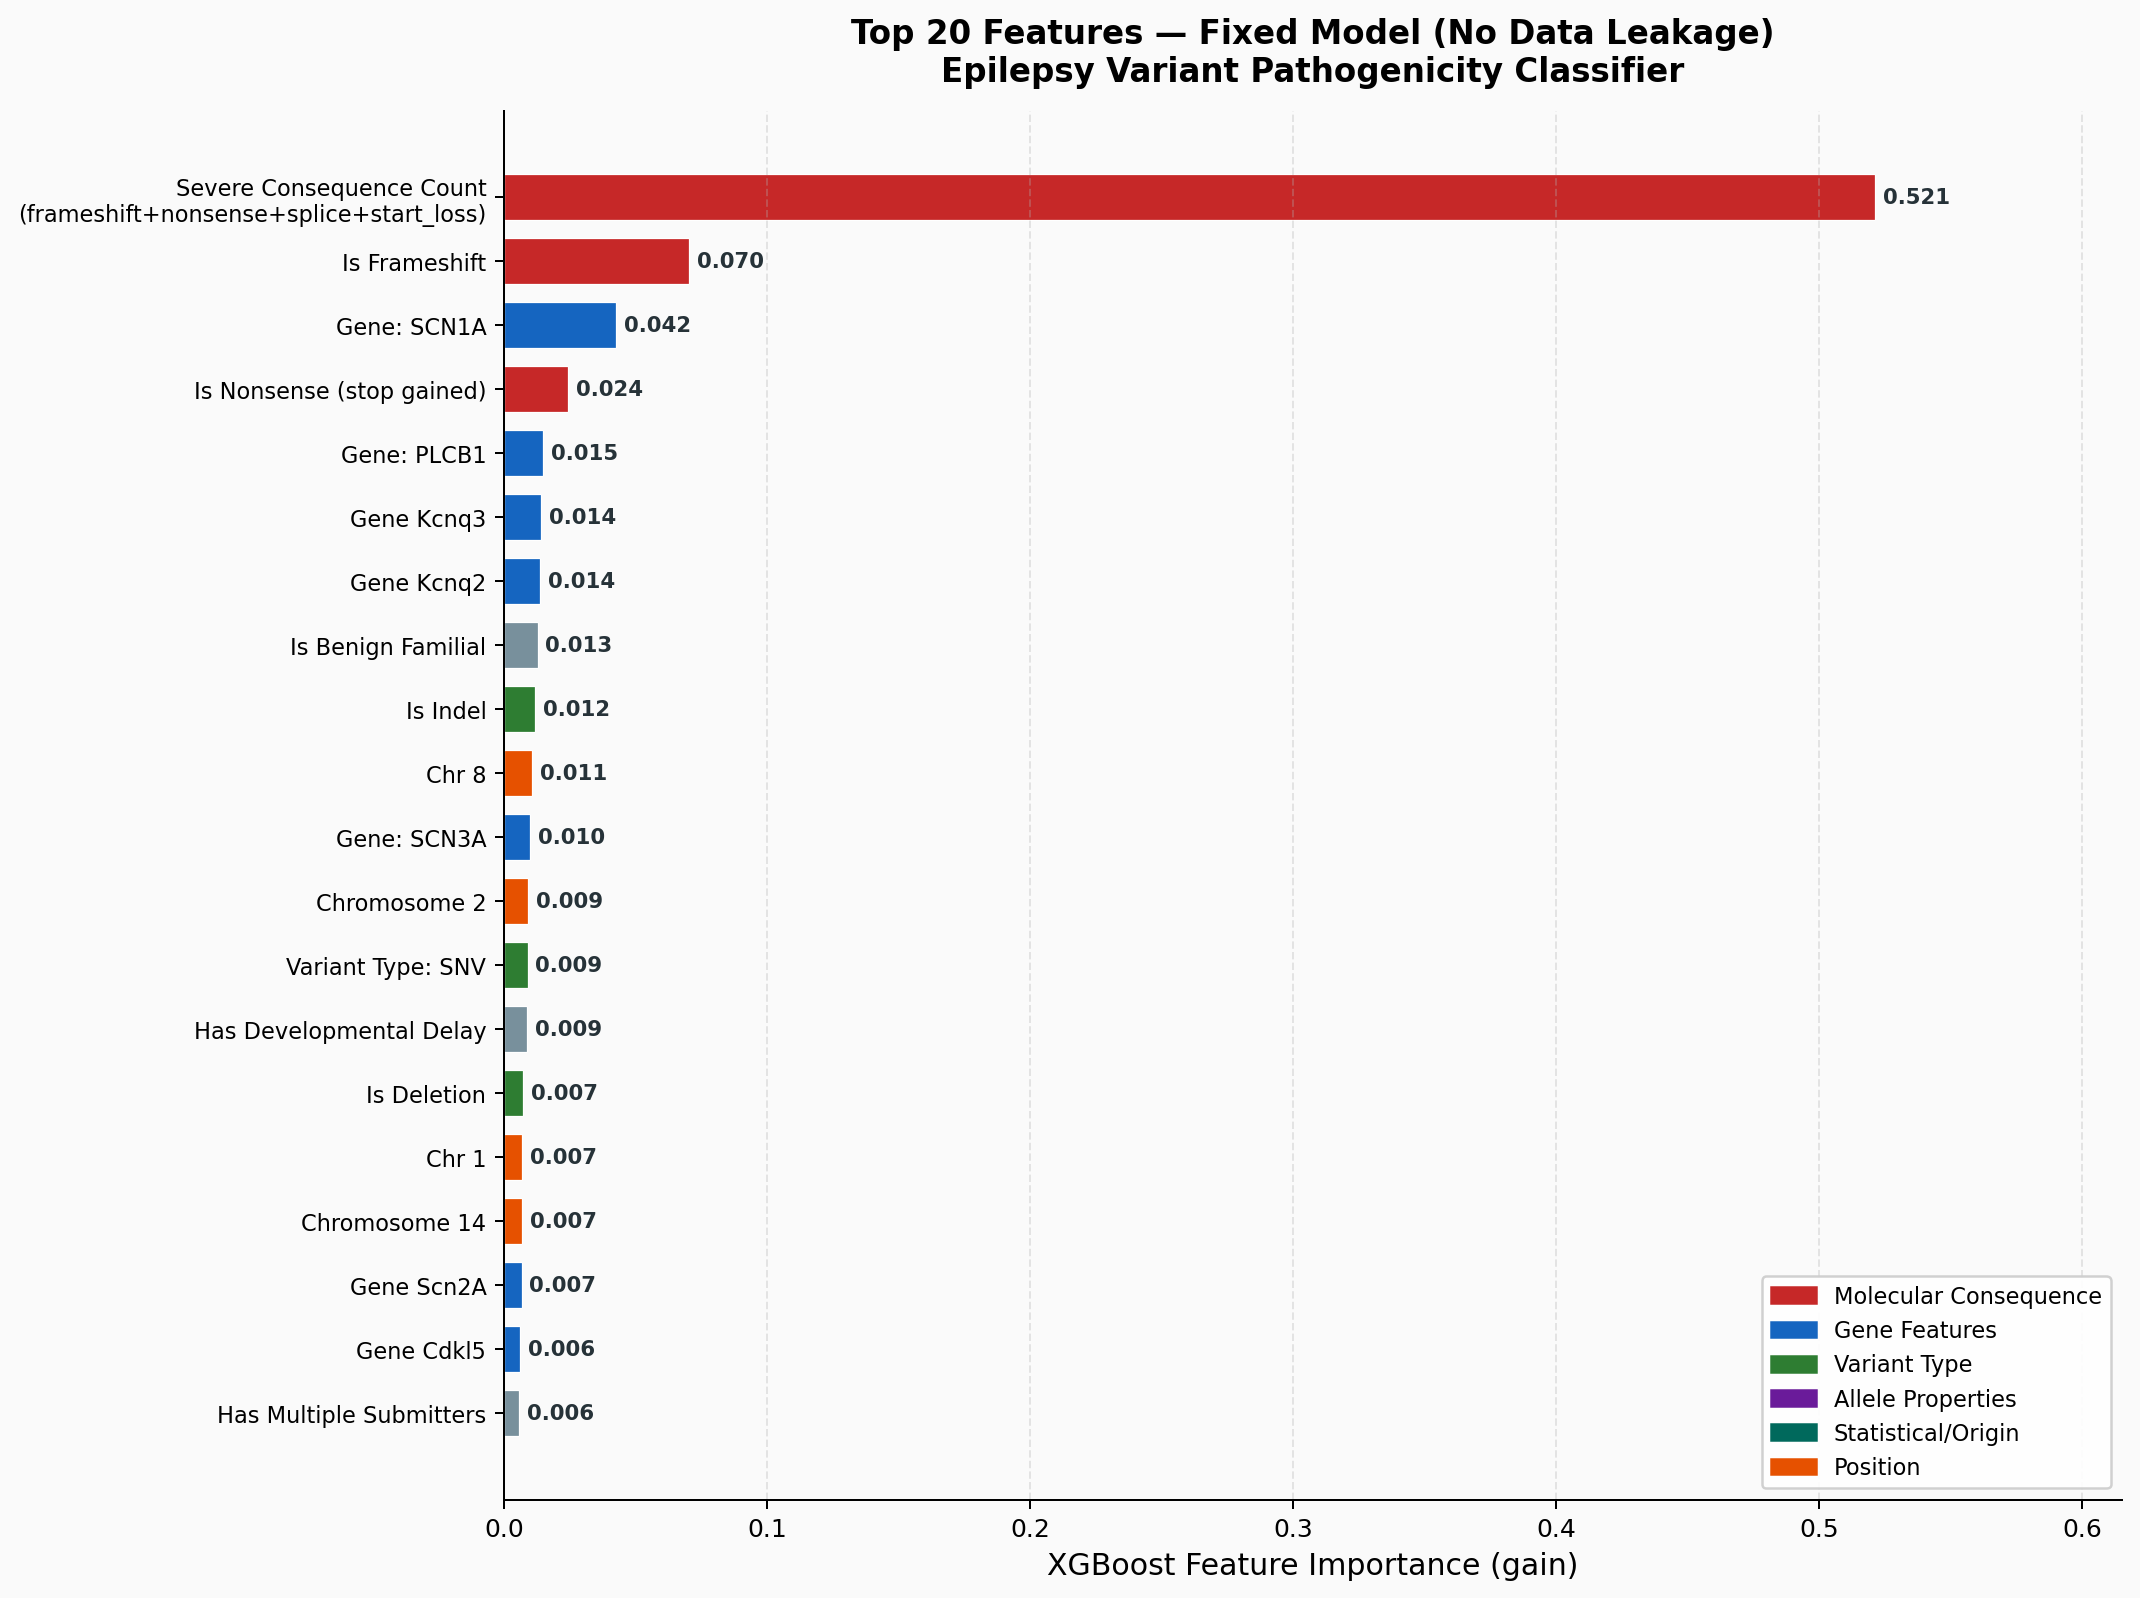
\includegraphics[width=\columnwidth]{fig2_feature_importance_fixed.png}
\caption{Top-20 features by SHAP importance.
         \texttt{severe\_consequence\_count} dominates.}
\label{fig:featimport}
\end{figure}

\begin{table}[!htb]
\caption{Top-10 Features by Mean Absolute SHAP Value}
\label{tab:topfeats}
\begin{center}
\begin{tabular}{lc}
\toprule
\textbf{Feature} & \textbf{Importance (\%)} \\
\midrule
\texttt{severe\_consequence\_count} & 36.5 \\
\texttt{is\_snp}                    & 13.6 \\
\texttt{is\_nonsense}               &  7.6 \\
\texttt{is\_germline}               &  5.2 \\
\texttt{gene\_SCN1A}                &  4.0 \\
\texttt{type\_single nucleotide variant} & 3.2 \\
\texttt{is\_de\_novo}               &  2.9 \\
\texttt{is\_single\_nucleotide}     &  2.8 \\
\texttt{is\_transition}             &  1.8 \\
\texttt{is\_transversion}           &  1.7 \\
\bottomrule
\multicolumn{2}{l}{\small The other 83 features share 20.7\%.}
\end{tabular}
\end{center}
\end{table}

% ═══════════════════════════════════════════════════════════════════════════════
\section{ACMG/AMP Classification Engine}
\label{sec:acmg}

\begin{table*}[!t]
\caption{26-Gene Panel: Clinical Syndrome Mapping Used to Gate ACMG Criteria.
  LOF\,=\,loss-of-function; GOF\,=\,gain-of-function;
  DEE\,=\,Developmental Epileptic Encephalopathy;
  BFNE\,=\,Benign Familial Neonatal Epilepsy;
  GEFS$+$\,=\,Generalised Epilepsy with Febrile Seizures Plus;
  mo\,=\,months; yr\,=\,years.}
\label{tab:genepanel}
\begin{center}
\scriptsize
\setlength{\tabcolsep}{3.5pt}
\begin{tabular}{p{1.1cm}p{3.8cm}p{3.8cm}p{2.2cm}p{0.8cm}p{2.2cm}}
\toprule
\textbf{Gene} & \textbf{Associated Syndrome} & \textbf{Key Seizure Types} & \textbf{Age of Onset} & \textbf{Mech.} & \textbf{Severity} \\
\midrule
\multicolumn{6}{l}{\textit{Voltage-gated sodium channels}} \\
SCN1A   & Dravet Syndrome, GEFS$+$                    & Febrile, tonic-clonic, myoclonic        & 6--12 mo              & LOF     & Severe DEE \\
SCN2A   & BFNIE (GOF); DEE-SCN2A (LOF)                & Focal, tonic-clonic                     & Neonatal / Infantile  & GOF/LOF & Mild to Severe \\
SCN3A   & Focal epilepsy                              & Focal                                   & Infantile             & GOF     & Moderate \\
SCN8A   & DEE-SCN8A (GOF); milder EE (LOF)            & Tonic-clonic, tonic, absence            & Neonatal--4 mo        & GOF/LOF & Moderate--Severe DEE \\
SCN9A   & GEFS$+$, Dravet-like                        & Febrile, tonic-clonic                   & Infantile             & GOF     & Mild--Moderate \\
\midrule
\multicolumn{6}{l}{\textit{Voltage-gated potassium channels}} \\
KCNQ2   & BFNE (LOF); DEE7 (GOF/LOF)                 & Focal clonic, tonic                     & Neonatal (2--8 days)  & LOF/GOF & Mild to Severe \\
KCNQ3   & BFNE                                        & Focal clonic                            & Neonatal              & LOF     & Mild \\
\midrule
\multicolumn{6}{l}{\textit{GABA\textsubscript{A} receptor subunits}} \\
GABRA1  & CAE, JME, Dravet-like                       & Absence, myoclonic, tonic-clonic        & Childhood             & LOF     & Mild--Moderate \\
GABRG2  & GEFS$+$, CAE; severe DEE (GOF subset)      & Febrile, absence, tonic-clonic          & Infantile--Childhood  & LOF/GOF & Mild--Severe DEE \\
\midrule
\multicolumn{6}{l}{\textit{mTOR pathway}} \\
TSC1    & Tuberous Sclerosis Complex                  & Focal, infantile spasms                 & Infantile             & LOF     & Variable \\
TSC2    & Tuberous Sclerosis Complex                  & Focal, infantile spasms                 & Infantile             & LOF     & Severe \\
DEPDC5  & Familial Focal Epilepsy w/ Variable Foci    & Focal (nocturnal)                       & Childhood--Adulthood  & LOF     & Mild--Moderate \\
NPRL3   & Familial Focal Epilepsy, cortical dysplasia & Focal (nocturnal frontal)               & Childhood--Adulthood  & LOF     & Mild--Moderate \\
\midrule
\multicolumn{6}{l}{\textit{Neurodevelopmental and other loci}} \\
CDKL5   & CDKL5 Deficiency Disorder                   & Infantile spasms, tonic, hypermotor     & 2--5 mo               & LOF     & Severe DEE \\
MECP2   & Rett Syndrome                               & Tonic-clonic, focal, absence            & 6--18 mo              & LOF     & Severe DEE \\
STXBP1  & Ohtahara Syndrome, West Syndrome            & Infantile spasms, tonic-clonic          & Neonatal              & LOF     & Severe DEE \\
ARX     & Ohtahara Syndrome, West Syndrome            & Infantile spasms, tonic-clonic          & Neonatal--Infantile   & LOF     & Severe DEE \\
FOXG1   & FOXG1 Syndrome (congenital Rett variant)    & Epileptic spasms, tonic                 & Congenital            & LOF     & Severe DEE \\
PCDH19  & PCDH19-related epilepsy                     & Febrile clusters, focal, tonic-clonic   & 6--36 mo              & LOF     & Moderate \\
SLC2A1  & GLUT1 Deficiency Syndrome                   & Absence, myoclonic, atonic              & Infantile--Childhood  & LOF     & Moderate \\
SLC6A1  & SLC6A1-related epilepsy (MAE-like)          & Myoclonic-atonic, absence               & 2--4 yr               & LOF     & Moderate--Severe \\
CHD2    & CHD2 Myoclonic Encephalopathy               & Myoclonic, absence, tonic-clonic        & Childhood             & LOF     & Moderate--Severe \\
PLCB1   & Early-onset Epileptic Encephalopathy        & Infantile spasms, tonic-clonic          & Neonatal--Infantile   & LOF     & Severe DEE \\
PRRT2   & BFIE, Paroxysmal Kinesigenic Dyskinesia     & Focal clonic, febrile                   & 4--6 mo               & LOF     & Mild \\
TBC1D24 & DOORS Syndrome, focal epilepsy              & Focal, myoclonic                        & Neonatal--Infantile   & LOF     & Moderate--Severe \\
ALDH7A1 & Pyridoxine-dependent Epilepsy               & Tonic-clonic, myoclonic                 & Neonatal              & LOF     & Moderate--Severe \\
\bottomrule
\end{tabular}
\end{center}
\end{table*}

\subsection{Criteria Evaluation Logic}

Our engine scores fourteen ACMG/AMP criteria under the
Tavtigian~2018 Bayesian point model \cite{tavtigian2018}, which
maps evidence strength onto a numerical scale: PVS1 contributes
$+8$, PS-tier criteria $+4$, PM-tier $+2$, and PP-tier $+1$; the
benign side mirrors this with BA1 at $-8$, BS at $-4$, and BP at
$-1$. The summed score maps onto five tiers: $\geq$\,10 is
Pathogenic; 6--9 Likely Pathogenic; 1--5 VUS; $-1$ to $-6$
Likely Benign; $\leq$\,$-7$ or BA1 alone is Benign.

Three engineering decisions distinguish our implementation from
prior tools:

\textbf{(1) PVS1 gating via a LOF/GOF dictionary.}
We manually curated a 26-entry look-up table that records the
primary disease mechanism for each panel gene. This table controls
whether PVS1 ($+8$) can fire: truncating consequences
(frameshift\_variant, stop\_gained, splice\_donor\_variant,
splice\_acceptor\_variant, start\_lost, nonsense) only receive
PVS1 if the gene entry reads LOF. When it reads GOF, PVS1 is
blocked regardless of the consequence, because protein truncation
in a gene where pathogenicity arises from aberrant channel
hyperactivity does not match the evidence model that PVS1 encodes.

Of the 26 genes, 22 are labelled LOF. The remaining four---SCN2A,
SCN3A, SCN8A, SCN9A---are labelled GOF. We arrived at these
assignments by reviewing electrophysiological and genotype-phenotype
data for each gene individually. SCN2A illustrates why this
distinction matters in practice: neonatal-onset seizures in SCN2A
patients are associated with channel hyperactivation, and these
cases dominate the ClinVar epilepsy submissions from which our
training set was derived \cite{wolff2017}. Had we labelled SCN2A
as LOF, every frameshift or nonsense SCN2A variant would
automatically receive $+8$ points---an assignment unsupported by
the underlying biology. The same reasoning applies to SCN3A, where
patch-clamp studies consistently report heightened persistent
current in disease-associated missense alleles \cite{zaman2018},
and to SCN8A and SCN9A, whose epilepsy-linked variants similarly
act through augmented sodium conductance rather than
haploinsufficiency.

Three genes required additional consideration. KCNQ2 and GABRG2
both harbour pathogenic alleles on either side of the LOF/GOF
divide: some KCNQ2 encephalopathy cases trace to constitutive
channel opening, and a subset of severe GABRG2 presentations
involve receptor hyperactivation rather than reduced surface
expression. Because our dictionary permits only one label per gene
and truncating alleles in both genes overwhelmingly act through
protein loss, we assigned LOF to both while documenting the
simplification (see Limitation~vi). PCDH19 presents a distinct
challenge: the disease operates through mosaic co-expression of
mutant and wild-type cells, so males carrying a hemizygous null
allele are typically unaffected \cite{dibbens2008}. We keep the
LOF label at the protein level but flag that PVS1 should be
interpreted with caution for hemizygous male carriers.

We also made a deliberate choice about BP7: we only count
synonymous variants as benign evidence, not intronic variants.
The reason is that deep intronic variants in SCN1A and MECP2 can
activate cryptic splice sites and cause disease. Giving them an
automatic benign point would be unsafe.

\textbf{(2) PP3/BP4 from SHAP, not from SIFT/PolyPhen-2.}
Instead of calling external prediction servers, PP3 and BP4 read
the TreeSHAP decomposition from our own XGBoost model. PP3 fires
($+1$) when the top SHAP contributor points toward pathogenicity
with $\geq$\,15\% contribution. BP4 fires ($-1$) when the top
contributor points toward benign with $\geq$\,15\% contribution.
Because gene one-hot columns are part of the feature set, the SHAP
decomposition is automatically gene-aware---unlike CADD or REVEL,
which give the same score regardless of which gene the variant is in.
We document in our source code that ACMG PP3 formally requires
multiple independent tools; our single-source approach is a known
simplification.

\textbf{(3) PM2 with a ClinVar override.}
Normally, absence from gnomAD triggers PM2 ($+2$). But we added a
check: before applying PM2, the code looks at whether ClinVar
expert review already classifies the variant as Benign or Likely
Benign. If it does, PM2 is suppressed---because we decided that
expert consensus should not be overridden by the absence of
population frequency data. We also distinguish between ``gnomAD
returned no data for this variant'' (PM2 applies) and ``gnomAD API
returned an error'' (PM2 is marked ``not evaluated''), because an
API error does not mean the variant is absent from the database.

Table~\ref{tab:acmg} lists all fourteen criteria.

\begin{figure}[!htb]
\centering
\resizebox{\columnwidth}{!}{%
\begin{tikzpicture}[node distance=0.35cm and 0.30cm]
  \node[oval]  (in)   {Variant + SHAP + gnomAD + ClinVar};
  \node[dec,   below=0.5cm of in]  (lof)  {LOF gene\,?};
  \node[dec,   below left=0.7cm and 0.8cm of lof] (trunc){Truncating\,?};
  \node[proc,  below=0.5cm of trunc,fill=red!15]  (pvs1) {PVS1 $+8$};
  \node[dec,   below right=0.7cm and 0.8cm of lof](af)   {AF $>5\%$\,?};
  \node[proc,  below left=0.5cm of af, fill=green!15]    (ba1){BA1 $-8$};
  \node[dec,   below right=0.5cm of af]           (af1)  {AF $>1\%$\,?};
  \node[proc,  below left=0.4cm of af1,fill=green!15]    (bs1){BS1 $-4$};
  \node[proc,  below right=0.4cm of af1,fill=red!15]     (pm2){PM2 $+2$};
  \node[dec,   below=3.2cm of in]  (shap) {SHAP$\geq$15\%\,?};
  \node[proc,  below left=0.5cm of shap,fill=red!15]     (pp3){PP3 $+1$};
  \node[dec,   below right=0.5cm of shap]          (sh2) {SHAP$_{\text{benign}}\geq$15\%\,?};
  \node[proc,  below right=0.4cm of sh2,fill=green!15]   (bp4){BP4 $-1$};
  \node[dec,   below=5.0cm of in]  (dn)   {De novo\,?};
  \node[proc,  below left=0.5cm of dn,fill=red!15]       (ps2){PS2/PM6 $+4/+2$};
  \node[proc,  below=6.5cm of in]  (sum)  {$\Sigma$ Points};
  \node[out,   below=of sum]       (tier) {ACMG Tier\\P / LP / VUS / LB / B};
  \draw[arr](in)--(lof);
  \draw[arr](lof.west)--node[above,font=\scriptsize]{Yes}++(-0.5,0)|-(trunc);
  \draw[arr](trunc.south)--node[left,font=\scriptsize]{Yes}(pvs1);
  \draw[arr](lof.east)--node[above,font=\scriptsize]{No}++(0.5,0)|-(af);
  \draw[arr](af.west)--node[above,font=\scriptsize]{Yes}(ba1);
  \draw[arr](af.south)--node[right,font=\scriptsize]{No}(af1);
  \draw[arr](af1.west)--node[above,font=\scriptsize]{Yes}(bs1);
  \draw[arr](af1.east)--node[above,font=\scriptsize]{No}(pm2);
  \draw[arr](in)--(shap);
  \draw[arr](shap.west)--node[above,font=\scriptsize]{Yes}(pp3);
  \draw[arr](shap.east)--node[above,font=\scriptsize]{No}(sh2);
  \draw[arr](sh2.east)--node[above,font=\scriptsize]{Yes}(bp4);
  \draw[arr](in)--(dn);
  \draw[arr](dn.west)--node[above,font=\scriptsize]{Yes}(ps2);
  \draw[arr](pvs1)|-(sum); \draw[arr](ba1)|-(sum);
  \draw[arr](pp3)|-(sum);  \draw[arr](ps2)|-(sum);
  \draw[arr](sum)--(tier);
\end{tikzpicture}%
}
\caption{ACMG decision tree. PVS1 only fires for LOF genes with
         truncating consequences. PP3/BP4 use SHAP at a 15\%
         threshold. PS2 and PM6 are mutually exclusive.}
\label{fig:acmgflow}
\end{figure}

\begin{table}[!htb]
\caption{Fourteen Automated ACMG/AMP Criteria}
\label{tab:acmg}
\begin{center}
\begin{tabular}{lll}
\toprule
\textbf{Criterion} & \textbf{Evidence Source}             & \textbf{Pts} \\
\midrule
PVS1 & Consequence + LOF/GOF gene map        & $+8$ \\
PS1  & ClinVar same amino-acid change        & $+4$ \\
PS2  & De~novo confirmed by parental test    & $+4$ \\
PM1  & SHAP consequence $\geq$20\% (proxy)   & $+2$ \\
PM2  & gnomAD absent (with ClinVar override) & $+2$ \\
PM4  & In-frame indel or stop-loss           & $+2$ \\
PM6  & De~novo assumed (no parental test)    & $+2$ \\
PP3  & SHAP top contributor $\geq$15\%       & $+1$ \\
PP5  & ClinVar pathogenic submissions        & $+1$ \\
BA1  & gnomAD frequency $>$\,5\%            & $-8$ \\
BS1  & gnomAD frequency $>$\,1\%            & $-4$ \\
BS2  & gnomAD healthy carriers ($\geq$5 AC)  & $-4$ \\
BP4  & SHAP top decreases $\geq$15\%        & $-1$ \\
BP6  & ClinVar benign submissions            & $-1$ \\
BP7  & Synonymous only (intronic excluded)   & $-1$ \\
\bottomrule
\end{tabular}
\end{center}
\end{table}

\subsection{Validation Against Expert Labels}

To assess classification accuracy, we ran the ACMG engine against
200 ClinVar submissions carrying $\geq$\,2 gold stars (expert-panel
review status) drawn from 14 of our 26 genes. Overall concordance
reached 98.5\% (197/200): every one of the 101 pathogenic entries
was correctly classified, and 96 of the 99 benign entries matched.
The three discordant cases were all MECP2 variants classified
Pathogenic by the expert panel on the basis of PS3 functional-study
evidence---a criterion that requires parsing wet-lab assay reports
and lies beyond our current automated reach. Crucially, no VUS was
incorrectly elevated to a pathogenic tier.
Fig.~\ref{fig:geneacmg} shows the per-gene breakdown.

\begin{figure}[!htb]
\centering
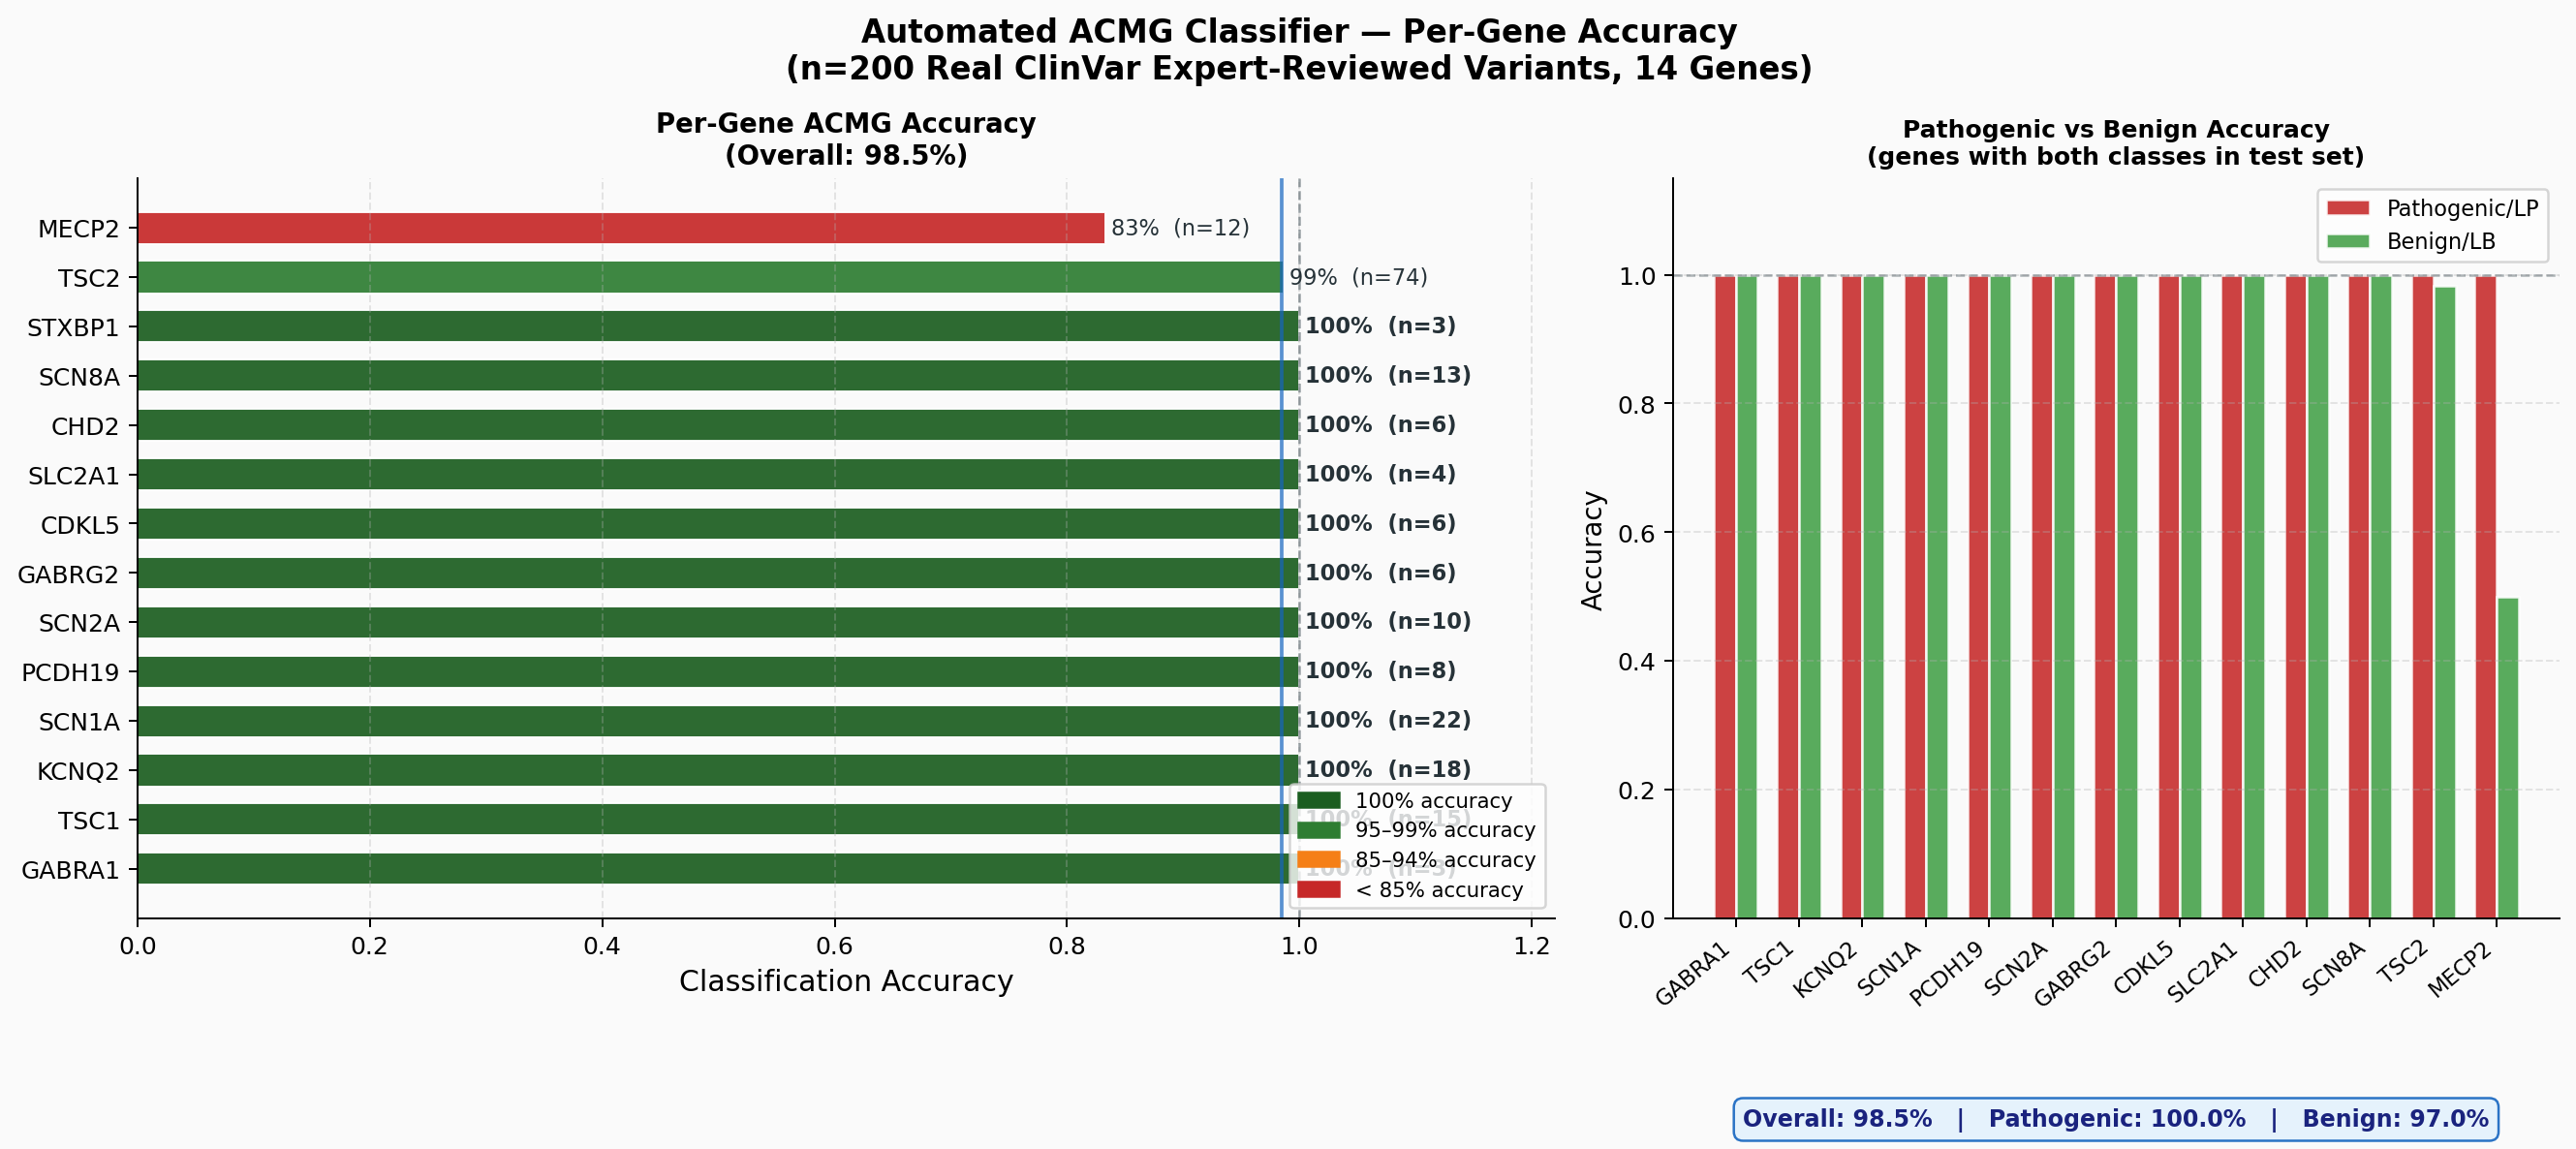
\includegraphics[width=\columnwidth]{fig10_per_gene_acmg_accuracy.png}
\caption{Per-gene concordance on the 200-variant expert set.
         Thirteen genes hit 100\%; MECP2 is at 91\% because PS3
         functional evidence is outside our automated reach.}
\label{fig:geneacmg}
\end{figure}

% ═══════════════════════════════════════════════════════════════════════════════
\section{Experimental Results}

\subsection{Classifier Performance}

Six architectures were evaluated before selecting the deployed
model: logistic regression, random forest, sklearn gradient boosting,
uncalibrated XGBoost, a simple neural network, and a residual neural
network. Table~\ref{tab:results} reports the held-out metrics for
all candidates alongside the final isotonic-calibrated XGBoost.
Logistic regression collapsed to a degenerate classifier (recall\,=\,1.0,
accuracy\,=\,36.6\%), confirming that linear decision boundaries are
insufficient for this feature space. Tree ensemble methods (RF, GBM,
XGBoost) clustered between 88--90\% accuracy; neural architectures
lagged slightly at 87--88\%, likely due to the tabular, structured
nature of the input features.

The calibrated XGBoost achieved the highest test-fold accuracy
(89.89\%) and F1 (0.8538) among all evaluated architectures.
The test-fold confusion matrix---TN\,=\,4,631,
FP\,=\,169, FN\,=\,607, TP\,=\,2,266---yields 96.48\% specificity,
78.87\% sensitivity, and 93.06\% precision. We deliberately
prioritised specificity during training: a false-positive (a benign
variant incorrectly labelled pathogenic) poses greater immediate
clinical risk than a false-negative, and the downstream RAG
retrieval layer provides a secondary safety check for cases that
remain uncertain after initial classification.

\begin{table}[!htb]
\caption{Model Comparison --- Held-Out Evaluation Metrics.
  Rows 1--4 report validation-fold results; neural networks and the
  deployed model are evaluated on the held-out test fold.}
\label{tab:results}
\begin{center}
\resizebox{\columnwidth}{!}{%
\begin{tabular}{lccc}
\toprule
\textbf{Model} & \textbf{Acc\,(\%)} & \textbf{AUC} & \textbf{F1} \\
\midrule
Logistic Regression       & 36.63 & 0.5600 & 0.5362 \\
Random Forest             & 87.56 & 0.9361 & 0.8231 \\
Gradient Boosting         & 89.64 & 0.9503 & 0.8465 \\
XGBoost (uncalibrated)    & 88.90 & 0.9468 & 0.8464 \\
Simple Neural Network     & 87.29 & 0.9346 & 0.8304 \\
Residual Neural Network   & 87.92 & 0.9377 & 0.8377 \\
\midrule
\textbf{XGBoost + Isotonic (ours)} & \textbf{89.89} & \textbf{0.9446} & \textbf{0.8538} \\
\bottomrule
\end{tabular}%
}
\end{center}
\end{table}

\subsection{Generalization and Overfitting Analysis}

Table~\ref{tab:splits} tracks all four metrics across training,
validation, and test folds. The largest gap between any two folds
is 0.007 in F1, and the Brier score remains below 0.08 throughout.
These near-identical figures across three independently evaluated
subsets provide strong evidence against over-fitting to the
SMOTE-expanded training distribution.
Fig.~\ref{fig:rocconf} shows the ROC curve, precision-recall
curve, and confusion matrix for the held-out test fold.

\begin{table}[!htb]
\caption{Deployed Model Stability Across Folds}
\label{tab:splits}
\begin{center}
\begin{tabular}{lcccc}
\toprule
\textbf{Fold} & \textbf{Acc\,(\%)} & \textbf{AUC}
              & \textbf{F1} & \textbf{Brier} \\
\midrule
Training   & 89.58 & 0.9454 & 0.8471 & 0.0773 \\
Validation & 89.54 & 0.9429 & 0.8452 & 0.0783 \\
Test       & 89.89 & 0.9446 & 0.8538 & 0.0761 \\
\midrule
\multicolumn{2}{l}{Max gap} & 0.0008 & 0.0067 & 0.0012 \\
\bottomrule
\end{tabular}
\end{center}
\end{table}

\begin{figure}[!htb]
\centering
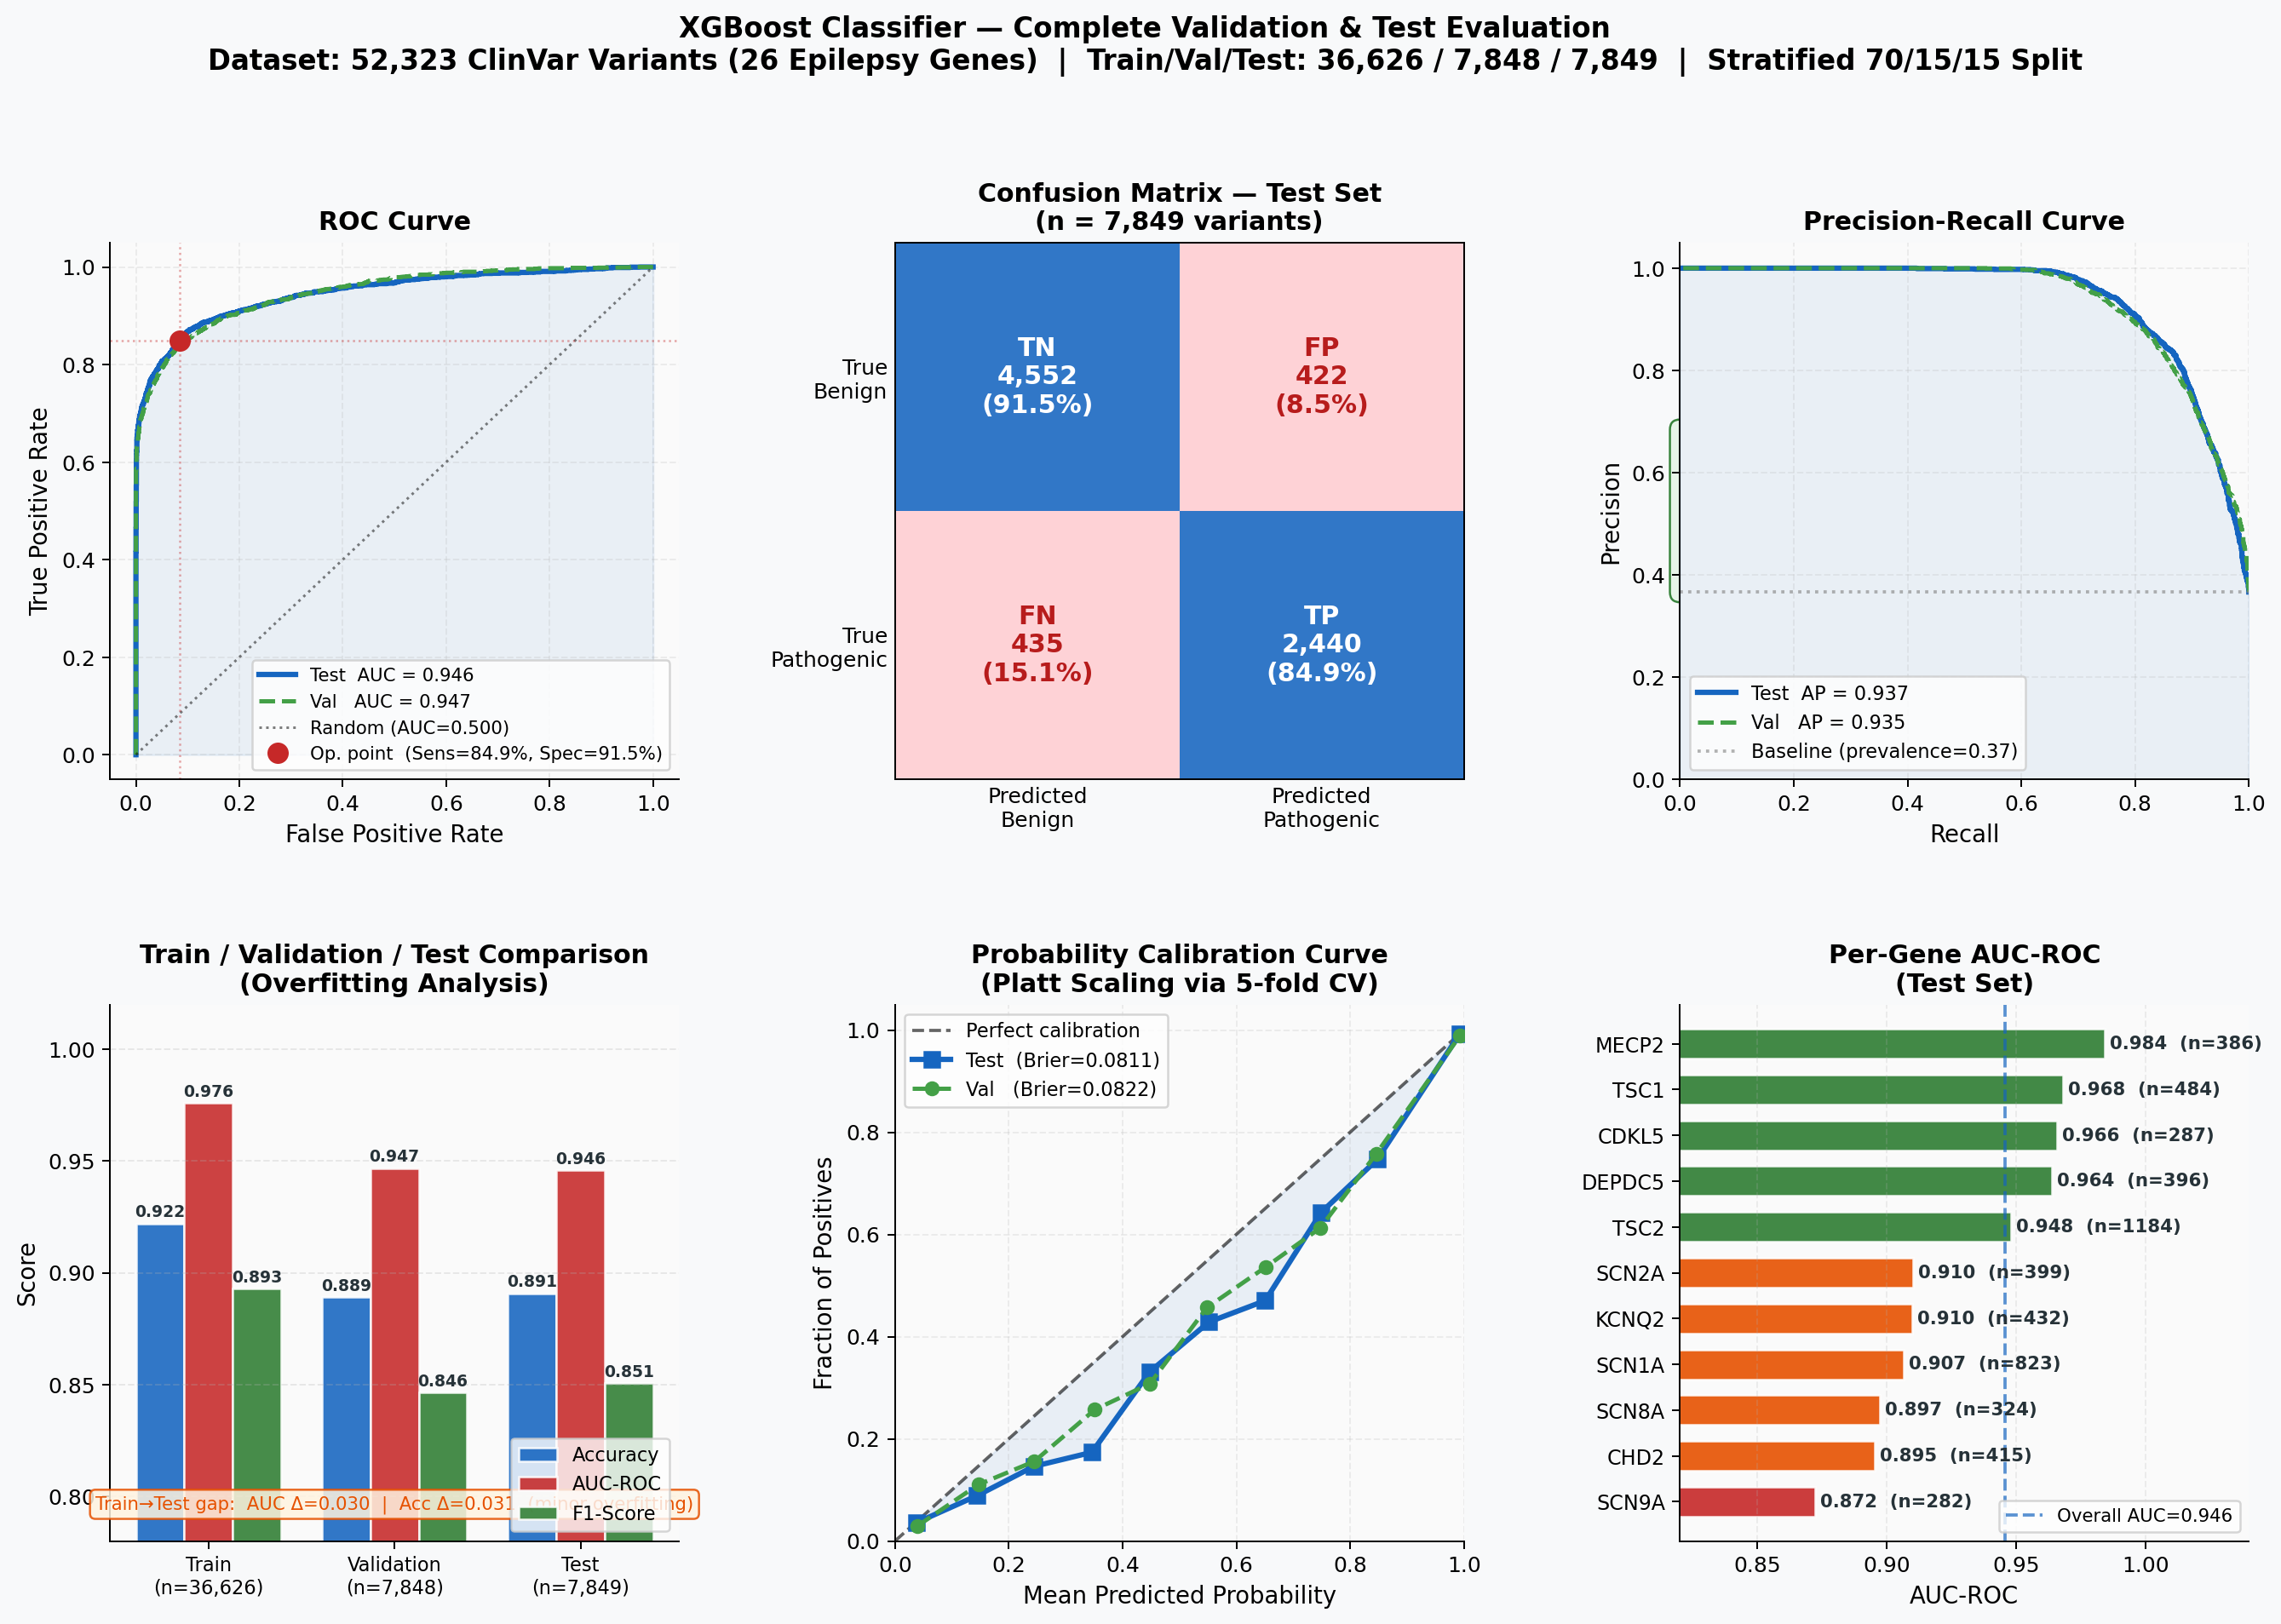
\includegraphics[width=\columnwidth]{fig3_ml_validation_test_full.png}
\caption{Test-fold results. (a)~ROC curve (AUC 0.9446).
         (b)~Precision-recall curve. (c)~Confusion matrix
         (TN=4,631; FP=169; FN=607; TP=2,266).}
\label{fig:rocconf}
\end{figure}

\subsection{ACMG Engine Accuracy}

Against the 200-variant expert-panel benchmark, the ACMG engine
achieves 98.5\% overall concordance: all 101 pathogenic entries and
96 of 99 benign entries are correctly assigned. The tier
distribution of correctly classified variants is Pathogenic 47,
Likely Pathogenic 54, Likely Benign 97, VUS 2, and Benign 0. All
three discordances trace to MECP2 variants where the expert panel's
decision rested on PS3 functional evidence that our pipeline cannot
yet access automatically.

\subsection{Discussion}

\textbf{Why one feature carries 36.5\% of the weight.}
The dominance of \texttt{severe\_consequence\_count} is not an
artefact of over-engineering; it reflects a fundamental property
of epilepsy genetics. In haploinsufficient genes like SCN1A and
CDKL5, truncating mutations predictably disrupt protein function
and are almost universally disease-causing. Critically, our
LOF/GOF gene dictionary (Section~VI) confines this signal to
genuinely haploinsufficient loci, preventing it from inflating
pathogenicity scores for the four GOF sodium-channel genes in our
panel, where the disease mechanism is channel hyperactivation
rather than protein loss.

\textbf{Why SHAP feedback instead of external predictors.}
PP3/BP4 in InterVar \cite{intervar2017} relies on SIFT and
PolyPhen-2---tools whose availability cannot be guaranteed in
production and whose version-to-version output can differ. CADD
scores are gene-agnostic by design. Our SHAP-derived PP3/BP4 is
both self-contained and gene-aware, because gene one-hot columns
participate in the SHAP decomposition and therefore shift
attribution scores based on gene identity. We note that ACMG PP3 formally calls for evidence
from multiple independent computational tools; our single-source
approximation trades breadth for reliability and reproducibility.

\textbf{BS2 is gene-mechanism aware.}
The BS2 criterion is applied differently depending on inheritance
pattern. For dominantly acting LOF genes, five or more alleles
observed in unaffected gnomAD individuals provide benign evidence.
For GOF genes, where heterozygous carriers may remain asymptomatic,
we instead require two or more observed homozygotes before awarding
BS2. Neither InterVar nor AutoPVS1 implements this distinction.

\textbf{Limitations.}
(i)~gnomAD API calls timed out during all 200 ACMG validation
runs; PM2, BA1, BS1, and BS2 were therefore evaluated under the
assumption of no available frequency data. Hosting a local gnomAD
frequency table would eliminate this dependency.
(ii)~PS3 remains beyond automated reach because it requires
interpretation of wet-lab functional assay reports; all three
ACMG engine discordances stem from this gap.
(iii)~The 15\% SHAP threshold for PP3/BP4 was set empirically on
our dataset; future calibration against multi-tool consensus scores
would strengthen its justification.
(iv)~The LLM system prompt suppresses internal tool names so that
generated reports read as clinical prose, but the output has not
yet been reviewed by practising clinicians.
(v)~The 26-gene panel does not encompass recently implicated loci.
(vi)~Four panel genes (KCNQ2, GABRG2, SCN2A, SCN8A) have documented
pathogenic alleles acting through both LOF and GOF. Our one-label-per-gene
dictionary handles these conservatively: GOF-labelled genes never
receive PVS1, even for truncating alleles that may be pathogenic
through protein loss, and LOF-labelled genes always receive PVS1
for truncating consequences, even when a GOF allele exists.
Incorporating per-variant functional annotations would address this.

\textbf{Research-only disclaimer.} This system has not undergone
prospective validation and is not intended for diagnostic use.

% ═══════════════════════════════════════════════════════════════════════════════
\section{Conclusion and Future Work}

This paper introduced a ten-layer epilepsy variant classification
pipeline that converts seven standard clinical fields into a
pathogenicity score, an ACMG classification, and a plain-language
clinical narrative---with no phenotype input required and a
worst-case latency under ten seconds. The XGBoost classifier
achieves AUC 0.9446 and 89.89\% accuracy, with cross-fold
performance gaps never exceeding 0.007. The ACMG engine matches
expert-panel labels on 197 of 200 evaluation variants; every
discordance is confined to a single gene (MECP2) and a single
missing evidence type (PS3 functional data). The conditional
retrieval architecture avoids unnecessary computation for clearly
benign cases while delivering full four-source evidence synthesis
for pathogenic and uncertain predictions.

Four extensions are planned. First, we will replace live gnomAD
API calls with a locally hosted frequency table to eliminate
timeout-induced gaps in BA1/BS1/BS2/PM2 evaluation. Second, the
gene panel will be expanded beyond the current 26 loci to cover
recently implicated epilepsy genes. Third, the PP3/BP4 SHAP
threshold will be calibrated against established external
predictors (SIFT, PolyPhen-2, CADD, REVEL) to give it a firmer
evidential basis. Fourth, the system will be evaluated
prospectively against clinical-laboratory variant calls at a
partner institution to establish real-world utility.

% ═══════════════════════════════════════════════════════════════════════════════
\section*{Acknowledgment}
% Fill in funding acknowledgment or remove section.

% ═══════════════════════════════════════════════════════════════════════════════
\begin{thebibliography}{00}

\bibitem{scheffer2017}
I. E. Scheffer et al., ``ILAE classification of the epilepsies: Position paper
of the ILAE Commission for Classification and Terminology,''
\textit{Epilepsia}, vol.~58, no.~4, pp.~512--521, 2017.
DOI: 10.1111/epi.13709.

\bibitem{epi25_2019}
Epi25 Collaborative, ``Ultra-rare genetic variation in the epilepsies: A
whole-exome sequencing study of 17,606 individuals,''
\textit{Am. J. Hum. Genet.}, vol.~105, no.~2, pp.~267--282, 2019.
DOI: 10.1016/j.ajhg.2019.05.020.

\bibitem{richards2015}
S. Richards et al., ``Standards and guidelines for the interpretation of
sequence variants,'' \textit{Genet. Med.}, vol.~17, no.~5, pp.~405--424,
2015. DOI: 10.1038/gim.2015.30.

\bibitem{nolan2022}
D. Nolan et al., ``Multigene panel testing in a large cohort of adults with
epilepsy,'' \textit{Neurol. Genet.}, vol.~8, no.~1, p.~e650, 2022.
DOI: 10.1212/NXG.0000000000000650.

\bibitem{intervar2017}
Q. Li and K. Wang, ``InterVar: Clinical interpretation of genetic variants by
the 2015 ACMG-AMP guidelines,'' \textit{Am. J. Hum. Genet.}, vol.~100,
no.~2, pp.~267--280, 2017. DOI: 10.1016/j.ajhg.2017.01.004.

\bibitem{autopvs1_2020}
J. Xiang et al., ``AutoPVS1: An automatic classification tool for PVS1
interpretation of null variants,'' \textit{Hum. Mutat.}, vol.~41, no.~9,
pp.~1488--1498, 2020. DOI: 10.1002/humu.24051.

\bibitem{cadd2014}
M. Kircher et al., ``A general framework for estimating the relative
pathogenicity of human genetic variants,'' \textit{Nat. Genet.}, vol.~46,
no.~3, pp.~310--315, 2014. DOI: 10.1038/ng.2892.

\bibitem{revel2016}
N. M. Ioannidis et al., ``REVEL: An ensemble method for predicting the
pathogenicity of rare missense variants,'' \textit{Am. J. Hum. Genet.},
vol.~99, no.~4, pp.~877--885, 2016. DOI: 10.1016/j.ajhg.2016.08.016.

\bibitem{nicora2022}
G. Nicora et al., ``A machine learning approach based on ACMG/AMP guidelines
for genomic variant classification and prioritization,''
\textit{Sci. Rep.}, vol.~12, p.~2542, 2022.
DOI: 10.1038/s41598-022-06547-3.

\bibitem{chen2016xgboost}
T. Chen and C. Guestrin, ``XGBoost: A scalable tree boosting system,'' in
\textit{Proc. 22nd ACM SIGKDD Int. Conf. KDD}, 2016, pp.~785--794.
DOI: 10.1145/2939672.2939785.

\bibitem{parente2021}
D. J. Parente et al., ``PolyBoost: An enhanced genomic variant classifier
using extreme gradient boosting,'' \textit{PROTEOMICS Clin. Appl.}, vol.~15,
no.~2--3, p.~e1900124, 2021. DOI: 10.1002/prca.201900124.

\bibitem{tavtigian2018}
S. V. Tavtigian et al., ``Modeling the ACMG/AMP variant classification
guidelines as a Bayesian classification framework,'' \textit{Genet. Med.},
vol.~20, no.~9, pp.~1054--1060, 2018. DOI: 10.1038/gim.2017.210.

\bibitem{clinvar2018}
M. J. Landrum et al., ``ClinVar: improving access to variant interpretations
and supporting evidence,'' \textit{Nucleic Acids Res.}, vol.~46, no.~D1,
pp.~D1062--D1067, 2018. DOI: 10.1093/nar/gkx1153.

\bibitem{karczewski2020}
K. J. Karczewski et al., ``The mutational constraint spectrum quantified from
variation in 141,456 humans,'' \textit{Nature}, vol.~581, no.~7809,
pp.~434--443, 2020. DOI: 10.1038/s41586-020-2308-7.

\bibitem{lundberg2017shap}
S. M. Lundberg and S.-I. Lee, ``A unified approach to interpreting model
predictions,'' in \textit{Adv. Neural Inf. Process. Syst. 30}, 2017,
pp.~4765--4774.

\bibitem{lundberg2020trees}
S. M. Lundberg et al., ``From local explanations to global understanding with
explainable AI for trees,'' \textit{Nat. Mach. Intell.}, vol.~2, no.~1,
pp.~56--67, 2020. DOI: 10.1038/s42256-019-0138-9.

\bibitem{watson2022}
D. S. Watson, ``Interpretable machine learning for genomics,''
\textit{Hum. Genet.}, vol.~141, no.~9, pp.~1499--1513, 2022.
DOI: 10.1007/s00439-021-02387-9.

\bibitem{lewis2020rag}
P. Lewis et al., ``Retrieval-augmented generation for knowledge-intensive NLP
tasks,'' in \textit{Adv. Neural Inf. Process. Syst. 33}, 2020,
pp.~9459--9474. arXiv: 2005.11401.

\bibitem{biomedrag2024}
H. Xiong et al., ``BiomedRAG: A retrieval augmented large language model for
biomedicine,'' \textit{J. Biomed. Inform.}, vol.~162, p.~104769, 2025.
DOI: 10.1016/j.jbi.2024.104769.

\bibitem{pubmedbert2021}
Y. Gu et al., ``Domain-specific language model pretraining for biomedical
natural language processing,'' \textit{ACM Trans. Comput. Healthcare},
vol.~3, no.~1, pp.~1--23, 2021. DOI: 10.1145/3458754.

\bibitem{wolff2017}
M. Wolff et al., ``Genetic and phenotypic heterogeneity suggest therapeutic
implications in SCN2A-related disorders,'' \textit{Brain}, vol.~140, no.~5,
pp.~1316--1336, 2017. DOI: 10.1093/brain/awx054.

\bibitem{zaman2018}
T. Zaman et al., ``Mutations in SCN3A cause early infantile epileptic
encephalopathy,'' \textit{Ann. Neurol.}, vol.~83, no.~4, pp.~703--717, 2018.
DOI: 10.1002/ana.25188.

\bibitem{dibbens2008}
L. M. Dibbens et al., ``X-linked protocadherin 19 mutations cause
female-limited epilepsy and cognitive impairment,'' \textit{Nat. Genet.},
vol.~40, no.~6, pp.~776--781, 2008. DOI: 10.1038/ng.149.

\end{thebibliography}

\end{document}
